% 若编译失败,且生成 .synctex(busy) 辅助文件,可能有两个原因:
% 1. 需要插入的图片不存在:Ctrl + F 搜索 'figure' 将这些代码注释/删除掉即可
% 2. 路径/文件名含中文或空格:更改路径/文件名即可

% --------------------- 文章宏包及相关设置 --------------------- %
% >> ------------------ 文章宏包及相关设置 ------------------ << %
% 设定文章类型与编码格式
\documentclass[UTF8]{article}		

% 物理实验报告所需的其它宏包
\usepackage{ulem}   % \uline 下划线支持
\usepackage{circuitikz} % 电路图 tikz 支持
\usepackage{pdfpages}   % 用于导入 pdf 文件

% 本 .tex 专属的宏定义
    \def\V{\ \mathrm{V}}
    \def\uV{\ \mu\mathrm{V}}
    \def\mV{\ \mathrm{mV}}
    \def\K{\ \mathrm{K}}
    \def\kV{\ \mathrm{KV}}
    \def\KV{\ \mathrm{KV}}
    \def\MV{\ \mathrm{MV}}
    \def\uA{\ \mu\mathrm{A}}
    \def\mA{\ \mathrm{mA}}
    \def\A{\ \mathrm{A}}
    \def\kA{\ \mathrm{KA}}
    \def\KA{\ \mathrm{KA}}
    \def\MA{\ \mathrm{MA}}
    \def\O{\ \Omega}
    \def\mO{\ \Omega}
    \def\kO{\ \mathrm{K}\Omega}
    \def\KO{\ \mathrm{K}\Omega}
    \def\MO{\ \mathrm{M}\Omega}
    \def\Hz{\ \mathrm{Hz}}
    \def\uF{\ \mu\mathrm{F}}
    \def\mF{\ \mathrm{mF}}
    \def\F{\ \mathrm{F}}
    \def\Re{\mathrm{\,Re}\,}
    \def\Im{\mathrm{\,Im}\,}
    \def\sinc{\mathrm{\,sinc}\,}

% 自定义宏定义
    \def\N{\mathbb{N}}
    \def\F{\mathbb{F}}
    \def\Z{\mathbb{Z}}
    \def\Q{\mathbb{Q}}
    \def\R{\mathbb{R}}
    \def\C{\mathbb{C}}
    \def\T{\mathbb{T}}
    \def\S{\mathbb{S}}
    %\def\A{\mathbb{A}}
    \def\I{\mathscr{I}}
    \def\d{\mathrm{d}}
    \def\p{\partial}


% 导入基本宏包
    \usepackage[UTF8]{ctex}     % 设置文档为中文语言
    \usepackage{hyperref}  % 宏包:自动生成超链接 (此宏包与标题中的数学环境冲突)
    \hypersetup{
        colorlinks=true,    % false:边框链接 ; true:彩色链接
        citecolor={blue},    % 文献引用颜色
        linkcolor={blue},   % 目录 (我们在目录处单独设置),公式,图表,脚注等内部链接颜色
        urlcolor={magenta},    % 网页 URL 链接颜色,包括 \href 中的 text
        % cyan 浅蓝色 
        % magenta 洋红色
        % yellow 黄色
        % black 黑色
        % white 白色
        % red 红色
        % green 绿色
        % blue 蓝色
        % gray 灰色
        % darkgray 深灰色
        % lightgray 浅灰色
        % brown 棕色
        % lime 石灰色
        % olive 橄榄色
        % orange 橙色
        % pink 粉红色
        % purple 紫色
        % teal 蓝绿色
        % violet 紫罗兰色
    }
    % \usepackage{docmute}    % 宏包:子文件导入时自动去除导言区,用于主/子文件的写作方式,\include{./51单片机笔记}即可。注:启用此宏包会导致.tex文件capacity受限。
    \usepackage{amsmath}    % 宏包:数学公式
    \usepackage{mathrsfs}   % 宏包:提供更多数学符号
    \usepackage{amssymb}    % 宏包:提供更多数学符号
    \usepackage{pifont}     % 宏包:提供了特殊符号和字体
    \usepackage{extarrows}  % 宏包:更多箭头符号 
    \usepackage{multicol}   % 宏包:支持多栏 

% 文章页面margin设置
    \usepackage[a4paper]{geometry}
        \geometry{top=0.75in}
        \geometry{bottom=0.75in}
        \geometry{left=0.75in}
        \geometry{right=0.75in}   % 设置上下左右页边距
        \geometry{marginparwidth=1.75cm}    % 设置边注距离(注释、标记等)

% 配置数学环境
    \usepackage{amsthm} % 宏包:数学环境配置
    % theorem-line 环境自定义
        \newtheoremstyle{MyLineTheoremStyle}% <name>
            {11pt}% <space above>
            {11pt}% <space below>
            {\kaishu}% <body font> 默认使用正文字体, \kaishu 为楷体
            {}% <indent amount>
            {\bfseries}% <theorem head font> 设置标题项为加粗
            {:\ \ }% <punctuation after theorem head>
            {.5em}% <space after theorem head>
            {\textbf{#1}\thmnumber{#2}\ \ (\,\textbf{#3}\,)}% 设置标题内容顺序
        \theoremstyle{MyLineTheoremStyle} % 应用自定义的定理样式
        \newtheorem{LineTheorem}{Theorem.\,}
    % theorem-block 环境自定义
        \newtheoremstyle{MyBlockTheoremStyle}% <name>
            {11pt}% <space above>
            {11pt}% <space below>
            {\kaishu}% <body font> 使用默认正文字体
            {}% <indent amount>
            {\bfseries}% <theorem head font> 设置标题项为加粗
            {:\\ \indent}% <punctuation after theorem head>
            {.5em}% <space after theorem head>
            {\textbf{#1}\thmnumber{#2}\ \ (\,\textbf{#3}\,)}% 设置标题内容顺序
        \theoremstyle{MyBlockTheoremStyle} % 应用自定义的定理样式
        \newtheorem{BlockTheorem}[LineTheorem]{Theorem.\,} % 使用 LineTheorem 的计数器
    % definition 环境自定义
        \newtheoremstyle{MySubsubsectionStyle}% <name>
            {11pt}% <space above>
            {11pt}% <space below>
            {}% <body font> 使用默认正文字体
            {}% <indent amount>
            {\bfseries}% <theorem head font> 设置标题项为加粗
            {:\\ \indent}% <punctuation after theorem head>
            {0pt}% <space after theorem head>
            {\textbf{#3}}% 设置标题内容顺序
        \theoremstyle{MySubsubsectionStyle} % 应用自定义的定理样式
        \newtheorem{definition}{}

%宏包:有色文本框(proof环境)及其设置
\usepackage{xcolor}    %设置插入的文本框颜色
    % rgb(4, 9, 103), rgb(5, 13, 164)
    % rgb(124, 131, 255), rgb(231, 232, 255)
    % rgb(255, 190, 190), rgb(255, 70, 70)
    \definecolor{stc}{RGB}{4, 10, 118}  % 设置各级标题结构颜色
\usepackage[strict]{changepage}     % 提供一个 adjustwidth 环境
\usepackage{framed}     % 实现方框效果
    % rgb(0, 0, 0), rgb(100, 100, 100)
    %#ECECED 为 0.93, 0.93, 0.93
    \definecolor{graybox_color}{rgb}{0.93, 0.93, 0.93} % 这里的 rbg 范围是 [0, 1]
    % 文本框颜色。修改此行中的 rgb 数值即可改变方框纹颜色,具体颜色的rgb数值可以在网站https://colordrop.io/ 中获得。(截止目前的尝试还没有成功过,感觉单位不一样)(找到喜欢的颜色,点击下方的小眼睛,找到rgb值,复制修改即可)
    \newenvironment{graybox}{%
    \def\FrameCommand{%
    \hspace{1pt}%
    {\color{gray}\small \vrule width 2pt}%
    {\color{graybox_color}\vrule width 4pt}%
    \colorbox{graybox_color}%
    }%
    \MakeFramed{\advance\hsize-\width\FrameRestore}%
    \noindent\hspace{-4.55pt}% disable indenting first paragraph
    \begin{adjustwidth}{}{7pt}%
    \vspace{2pt}\vspace{2pt}%
    }
    {%
    \vspace{2pt}\end{adjustwidth}\endMakeFramed%
    }

    \definecolor{bluebox_ruleColor}{rgb}{0.49, 0.51, 1} % 文本框颜色。修改此行中的 rgb 数值即可改变方框纹颜色,具体颜色的rgb数值可以在网站https://colordrop.io/ 中获得。(截止目前的尝试还没有成功过,感觉单位不一样)(找到喜欢的颜色,点击下方的小眼睛,找到rgb值,复制修改即可)
    \definecolor{bluebox_backgroundColor}{rgb}{0.93, 0.93, 1}
    \newenvironment{bluebox}{%
    \def\FrameCommand{%
    \hspace{1pt}%
    {\color{bluebox_ruleColor}\small \vrule width 2pt}%
    {\color{bluebox_backgroundColor}\vrule width 4pt}% 4pt 缩进比较合适
    \colorbox{bluebox_backgroundColor}%
    }%
    \MakeFramed{\advance\hsize-\width\FrameRestore}%
    \noindent\hspace{-4.55pt}% disable indenting first paragraph
    \begin{adjustwidth}{}{7pt}%
    \vspace{2pt}\vspace{2pt}%
    }
    {%
    \vspace{2pt}\end{adjustwidth}\endMakeFramed%
    }

    \definecolor{redbox_ruleColor}{rgb}{1, 0.27, 0.27} % 文本框颜色。修改此行中的 rgb 数值即可改变方框纹颜色,具体颜色的rgb数值可以在网站https://colordrop.io/ 中获得。(截止目前的尝试还没有成功过,感觉单位不一样)(找到喜欢的颜色,点击下方的小眼睛,找到rgb值,复制修改即可)
    \definecolor{redbox_backgroundColor}{rgb}{1, 0.90, 0.90}
    \newenvironment{redbox}{%
    \def\FrameCommand{%
    \hspace{1pt}%
    {\color{redbox_ruleColor}\small \vrule width 2pt}%
    {\color{redbox_backgroundColor}\vrule width 4pt}% 4pt 缩进比较合适
    \colorbox{redbox_backgroundColor}%
    }%
    \MakeFramed{\advance\hsize-\width\FrameRestore}%
    \noindent\hspace{-4.55pt}% disable indenting first paragraph
    \begin{adjustwidth}{}{7pt}%
    \vspace{2pt}\vspace{2pt}%
    }
    {%
    \vspace{2pt}\end{adjustwidth}\endMakeFramed%
    }

% 外源代码插入设置
    % matlab 代码插入设置
    \usepackage{matlab-prettifier}
        \lstset{style=Matlab-editor}    % 继承 matlab 代码高亮 , 此行不能删去
    \usepackage[most]{tcolorbox} % 引入tcolorbox包 
    \usepackage{listings} % 引入listings包
        \tcbuselibrary{listings, skins, breakable}
        \newfontfamily\codefont{Consolas} % 定义需要的 codefont 字体
        \lstdefinestyle{MatlabStyle_inc}{   % 插入代码的样式
            language=Matlab,
            basicstyle=\footnotesize\ttfamily\codefont,    % ttfamily 确保等宽 
            breakatwhitespace=false,
            breaklines=true,
            captionpos=b,
            keepspaces=true,
            numbers=left,
            numbersep=15pt,
            showspaces=false,
            showstringspaces=false,
            showtabs=false,
            tabsize=2,
            xleftmargin=15pt,   % 左边距
            %frame=single, % single 为包围式单线框
            frame=shadowbox,    % shadowbox 为带阴影包围式单线框效果
            %escapeinside=``,   % 允许在代码块中使用 LaTeX 命令 (此行无用)
            %frameround=tttt,    % tttt 表示四个角都是圆角
            framextopmargin=0pt,    % 边框上边距
            framexbottommargin=0pt, % 边框下边距
            framexleftmargin=5pt,   % 边框左边距
            framexrightmargin=5pt,  % 边框右边距
            rulesepcolor=\color{red!20!green!20!blue!20}, % 阴影框颜色设置
            %backgroundcolor=\color{blue!10}, % 背景颜色
        }
        \lstdefinestyle{MatlabStyle_src}{   % 插入代码的样式
            language=Matlab,
            basicstyle=\small\ttfamily\codefont,    % ttfamily 确保等宽 
            breakatwhitespace=false,
            breaklines=true,
            captionpos=b,
            keepspaces=true,
            numbers=left,
            numbersep=15pt,
            showspaces=false,
            showstringspaces=false,
            showtabs=false,
            tabsize=2,
        }
        \newtcblisting{matlablisting}{
            %arc=2pt,        % 圆角半径
            % 调整代码在 listing 中的位置以和引入文件时的格式相同
            top=0pt,
            bottom=0pt,
            left=-5pt,
            right=-5pt,
            listing only,   % 此句不能删去
            listing style=MatlabStyle_src,
            breakable,
            colback=white,   % 选一个合适的颜色
            colframe=black!0,   % 感叹号后跟不透明度 (为 0 时完全透明)
        }
        \lstset{
            style=MatlabStyle_inc,
        }

% table 支持
    \usepackage{booktabs}   % 宏包:三线表
    \usepackage{tabularray} % 宏包:表格排版
    \usepackage{longtable}  % 宏包:长表格

% figure 设置
    \usepackage{graphicx}  % 支持 jpg, png, eps, pdf 图片 
    \usepackage{svg}       % 支持 svg 图片
        \svgsetup{
            % 指向 inkscape.exe 的路径
            inkscapeexe = C:/aa_MySame/inkscape/bin/inkscape.exe, 
            % 一定程度上修复导入后图片文字溢出几何图形的问题
            inkscapelatex = false                 
        }
    \usepackage{subcaption} % 用于子图和小图注  

% 图表进阶设置
    \usepackage{caption}    % 图注、表注
        \captionsetup[figure]{name=图}  
        \captionsetup[table]{name=表}
        \captionsetup{
            labelfont=bf, % 设置标签为粗体
            textfont=bf,  % 设置文本为粗体
            font=small  
        }
    \usepackage{float}     % 图表位置浮动设置 
    \usepackage{etoolbox} % 用于保证图注表注的数学字符为粗体
        \AtBeginEnvironment{figure}{\boldmath} % 图注中的数学字符为粗体
        \AtBeginEnvironment{table}{\boldmath}  % 表注中的数学字符为粗体
        \AtBeginEnvironment{tabular}{\unboldmath}   % 保证表格中的数学字符不受额外影响

% 圆圈序号自定义
    \newcommand*\circled[1]{\tikz[baseline=(char.base)]{\node[shape=circle,draw,inner sep=0.8pt, line width = 0.03em] (char) {\bfseries #1};}}   % TikZ solution

% 列表设置
    \usepackage{enumitem}   % 宏包:列表环境设置
        \setlist[enumerate]{
            label=(\arabic*) ,   % 设置序号样式为加粗的 (1) (2) (3)
            ref=\arabic*, % 如果需要引用列表项,这将决定引用格式(这里仍然使用数字)
            itemsep=0pt, parsep=0pt, topsep=0pt, partopsep=0pt, leftmargin=3.5em} 
        \setlist[itemize]{itemsep=0pt, parsep=0pt, topsep=0pt, partopsep=0pt, leftmargin=3.5em}
        \newlist{circledenum}{enumerate}{1} % 创建一个新的枚举环境  
        \setlist[circledenum,1]{  
            label=\protect\circled{\arabic*}, % 使用 \arabic* 来获取当前枚举计数器的值,并用 \circled 包装它  
            ref=\arabic*, % 如果需要引用列表项,这将决定引用格式(这里仍然使用数字)
            itemsep=0pt, parsep=0pt, topsep=0pt, partopsep=0pt, leftmargin=3.5em
        }  

% 其它设置
    % 脚注设置
        \renewcommand\thefootnote{\ding{\numexpr171+\value{footnote}}}
    % 参考文献引用设置
        \bibliographystyle{unsrt}   % 设置参考文献引用格式为unsrt
        \newcommand{\upcite}[1]{\textsuperscript{\cite{#1}}}     % 自定义上角标式引用
    % 文章序言设置
        \newcommand{\cnabstractname}{序言}
        \newenvironment{cnabstract}{%
            \par\Large
            \noindent\mbox{}\hfill{\bfseries \cnabstractname}\hfill\mbox{}\par
            \vskip 2.5ex
            }{\par\vskip 2.5ex}

% 文章默认字体设置
    \usepackage{fontspec}   % 宏包:字体设置
        \setmainfont{SimSun}    % 设置中文字体为宋体字体
        \setCJKmainfont[AutoFakeBold=3]{SimSun} % 设置加粗字体为 SimSun 族,AutoFakeBold 可以调整字体粗细
        \setmainfont{Times New Roman} % 设置英文字体为Times New Roman

% 各级标题自定义设置
    \usepackage{titlesec}   
        % section标题自定义设置 
        \titleformat{\section}[hang]{\normalfont\Large\bfseries\boldmath}{\thesection}{8pt}{}
        % subsection 标题自定义设置
        \titleformat{\subsection}[hang]{\normalfont\large\bfseries\boldmath}{\thesubsection}{8pt}{}
        \titlespacing*{\subsection}{0pt}{10pt}{6pt} % 控制上下间距


% --------------------- 文章宏包及相关设置 --------------------- %
% >> ------------------ 文章宏包及相关设置 ------------------ << %




% ------------------------ 文章信息区 ------------------------ %
% ------------------------ 文章信息区 ------------------------ %
% 页眉页脚设置
\usepackage{fancyhdr}   %宏包:页眉页脚设置
    \pagestyle{fancy}
    \fancyhf{}
    \cfoot{\thepage}
    \renewcommand\headrulewidth{1pt}
    \renewcommand\footrulewidth{0pt}
    %\rhead{《线性电路实验》实验报告}    
    \lhead{\small \faGithub\ \href{https://github.com/YiDingg/UCAS-LinearCircuitExperiment}{\color{black} https://github.com/YiDingg/UCAS-LinearCircuitExperiment}}


    \graphicspath{{../}}   % 修改主文件图像路径,使得子文件能够直接使用相对路径,而不是从 assets 开始索引

    \usepackage{fontawesome}    % 宏包:更多符号与图标 (用于插入 GitHub 图标等)



%%%%%%%%%%%%%%%%%%%%%%%%%%%%%%%%%%%%%%%%%%%%%%%%%%%%%%%%%%%%%%%%
% 仅需修改左页眉、实验名称、实验日期
%%%%%%%%%%%%%%%%%%%%%%%%%%%%%%%%%%%%%%%%%%%%%%%%%%%%%%%%%%%%%%%%


%%%%%%%%%%%%%%%%%% 1. 修改左页眉内容 %%%%%%%%%%%%%%%%%%
\lhead{LCE-01 二极管 (2025.03.28, 丁毅)}

% 开始编辑文章
\begin{document}
\begin{center}\large
    \vspace*{-0.8cm}
    \noindent{\huge\bfseries《\ \ 线\ \ 性\ \ 电\ \ 路\ \ 实\ \ 验\ \ \ 》\ \ 实\ \ 验\ \ 报\ \ 告 }
    \\\vspace{0.1cm}
    \noindent{
    {\bfseries 
%
%%%%%%%%%%%%%%%%%% 2. 修改实验名称 %%%%%%%%%%%%%%%%%%
    实验名称:\uline{\hspace{2.2cm} 二极管 \hspace{2.2cm}}
%%%%%%%%%%%%%%%%%% 2. 修改实验名称 %%%%%%%%%%%%%%%%%%
%
    }\hspace{0.4cm}
    指导教师:\uline{\hspace{0.8cm}王东雷\ \ \ \  \ df4dac@sina.com     \hspace{0.8cm}}
    }
    \\\vspace{0.1cm}
    \noindent
    {
    姓名:\uline{\,\,\,丁毅\,\,\,}\hspace{0.2cm}
    学号:\uline{\,\,\,{ 2023K8009908031}\,\,\,}\hspace{0.2cm}
    班级/专业:\uline{\,\,\,{2308/电子信息}\,\,\,}\hspace{0.2cm}
    分组序号:\uline{\,\,\,{2-06}\,\,\,}
    }
    \\\vspace{0.1cm}
    \noindent{
%
%%%%%%%%%%%%%%%%%% 3. 修改实验日期 %%%%%%%%%%%%%%%%%%
    实验日期:\uline{\,\,{2025.03.28}\,\,}\hspace{0.2cm}
%%%%%%%%%%%%%%%%%% 3. 修改实验日期 %%%%%%%%%%%%%%%%%%
%
    实验地点:\uline{\,\,\,教学楼{ 607}\,\,\,}\hspace{0.2cm}
    是否调课/补课:\uline{\hspace{0.26cm}否 \hspace{0.26cm}}\hspace{0.2cm}
    成绩:\uline{\hspace{2cm}}
    }
\end{center}
\vspace{-0.4cm}
\noindent\rule{\textwidth}{0.075em}   % 分割线
\vspace{-1.0cm}

% 生成目录
\setcounter{tocdepth}{3}  % 目录深度为 2(不显示 subsubsection)
\noindent\tableofcontents\thispagestyle{fancy}   % 显示页码、页眉等

% ------------------------ 文章信息区 ------------------------ %
% ------------------------ 文章信息区 ------------------------ %



%%%%%%%%%%%%%%%%%%%%%%%%%%%%%%%%%%%%%%%%%%%%%%%%%%%%%%%%%%%%%%%%%%%%%%%%%%%%%%%%%
%%%%%%%%%%%%%%%%%%%%%%%%%%%%%%%%% 下面是正文内容 %%%%%%%%%%%%%%%%%%%%%%%%%%%%%%%%%
%%%%%%%%%%%%%%%%%%%%%%%%%%%%%%%%%%%%%%%%%%%%%%%%%%%%%%%%%%%%%%%%%%%%%%%%%%%%%%%%%

\section{实验目的}

\begin{enumerate}
    \item 理解数字万用表原理,精度指标,不同功能的阻抗以及对电路的影响;
    \item 理解基础测量仪器,了解示波器、万用表、电源和信号源的用法;
    \item 理解二极管的种类以及主要参数,用万用表简单测量二极管;
    \item 加深理解理论课程,熟悉二极管整流滤波电路的波形以及参数;
    \item 简单焊接练习;
    \item 实测电容滤波电流波形,理解电容滤波对电网的影响,初步建立功率因数的概念。
\end{enumerate}


\section{实验仪器}

\begin{enumerate}
    \item 数字万用表: Unit UT61E (C190241394)
    \item 数字示波器: RIGOL 200MSO2202A (DS2F192200361)
    \item 信号发生器: Goodwill AFG-22225 (GER910370)
    \item 数字直流电源: GWINSTEK GPD-3303S (GES813705)
    \item 普通硅整流管 1N4007、硅开关管 1N4148、锗二极管 1N60、肖特基二极管 1N5819、稳压二极管C6V2、温度补偿稳压二极管 2DW234、各颜色发光二极管;以及电阻、电容、变压器、导线等若干。
\end{enumerate}

\section{实验内容及实验结果}

\subsection{二极管导通压降}

一种方法是直接万用表的“二极管”档进行测量。此时,万用表可以看作一个电流比较小的恒流源(约 1 mA ),正确连接二极管时,会使二极管导通(产生压降),并显示二极管的压降数值。需要注意的是,多数万用表只能显示 2 V 以内的压降值,如果二极管的压降超过 2 V ,则会显示 OL (Over Load) 或其它表示超出量程的符号。

因此,为了能够测量高压降的二极管(例如蓝色 LED 灯),我们使用 DC Power Supply + 1 k$\Omega$ 电阻进行测量。电阻用于限流,二极管的压降由万用表电压档测量,电流由 DC Power Supply 直接读出。

实验中测得的数据如下表所示,其中 $V_D$ 指二极管的正向压降,$I_D$ 指正向电流。

\begin{table}[H]\centering
    %\renewcommand{\arraystretch}{1.5} % 调整行间距为 1.5 倍
    %\setlength{\tabcolsep}{1.5mm} % 调整列间距
    \caption{二极管导通压降实验数据}
    \label{二极管导通压降实验数据}
\begin{tabular}{lll}\toprule
    Diode & $V_D$ (V) & $I_D$ (mA) \\
    \midrule
    LED (Red)           & 1.9772 & 11 \\
    LED (Blue)          & 3.074  & 12 \\
    LED (Green)         & 1.9842 & 7 \\
    LED (Yellow)        & 1.9794 & 9 \\
    LED (White)         & 2.776  & 10 \\
    1N5819 (Schottky)   & 0.2697 & 17 \\
    1N4007 (General)    & 0.6855 & 6 \\
    2DW234 (Zener)      & -6.318  & -8 \\
    ST60P (Ge)          & 0.5604 & 19 \\
    BZX55C6V2 (Zener)   & -6.246  & -15 \\
    BZX55C6V2 (Zener)   & 0.8156 & 21 \\
    \bottomrule
\end{tabular}
\end{table}

\noindent 注:由于我们使用的是 DC Power Supply + 限流电阻进行测试,不存在类似于万用表“导通压降测量范围在 0 $\sim$ 2 V” 的问题。

\subsection{二极管伏安特性曲线}

利用信号发生器作为激励,经过合适的测量电路,利用示波器的 X-Y 模式绘制二极管的伏安特性曲线。其中,信号源作为激励,变压器提供隔离作用,二极管电流通过 1 $\Omega$ 电阻检测。测量电路如下图所示:

\begin{figure}[H]\centering
    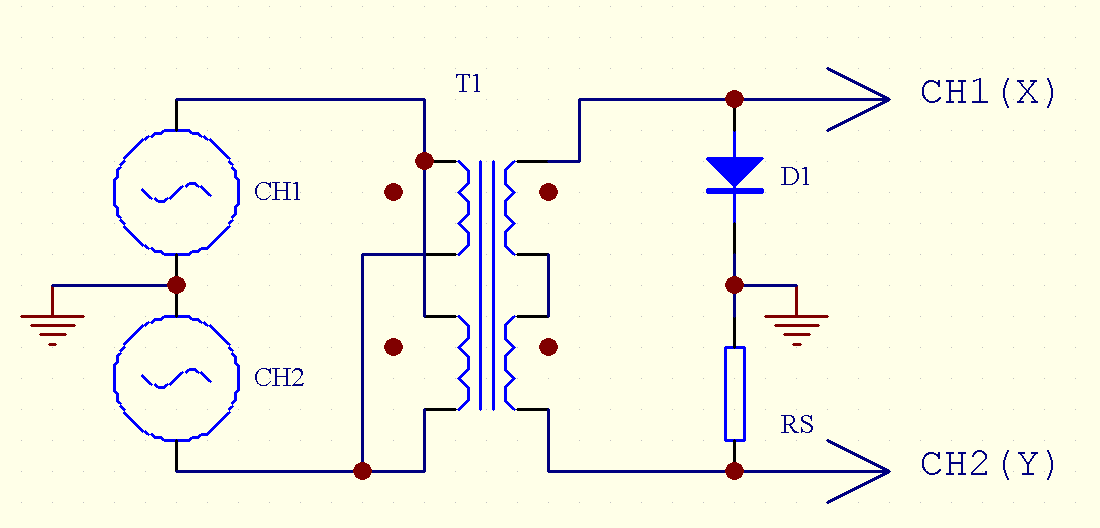
\includegraphics[width=0.5\columnwidth]{LCE-01-二极管/assets/实验原理/二极管伏安特性曲线.png}
    \caption{二极管伏安特性曲线测量电路}
\end{figure}

我们分别测量了 1N5819 (Schottky) 、 LED (Blue) 和 LED (Green) 的特性曲线,所用电流感应电阻 $R_{sense} = 1 \ \mathrm{k}\Omega$,测量结果如下图所示。

\begin{figure}[H]\centering
    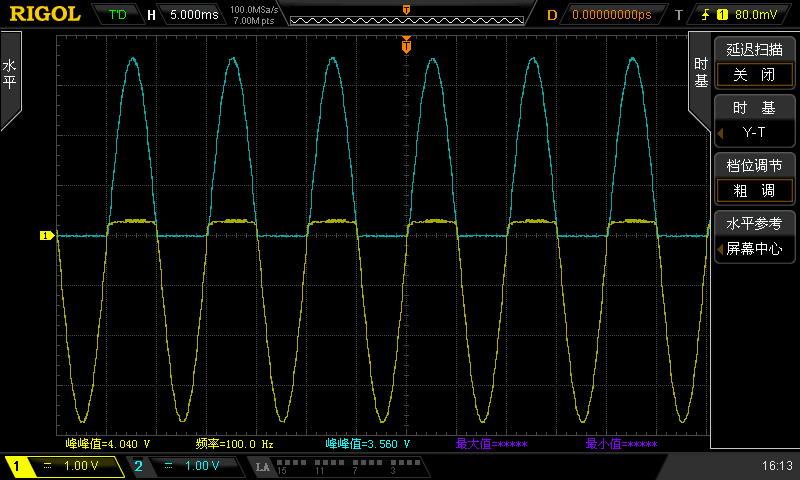
\includegraphics[width=\columnwidth]{LCE-01-二极管/assets/二极管伏安特性曲线/1N5819 Schottky Y-T.png}
    \caption{1N5819 (Schottky) 伏安特性曲线 (Y-T mode), $R_{sense} = 1 \ \mathrm{k}\Omega$}
\end{figure}

\begin{figure}[H]\centering
    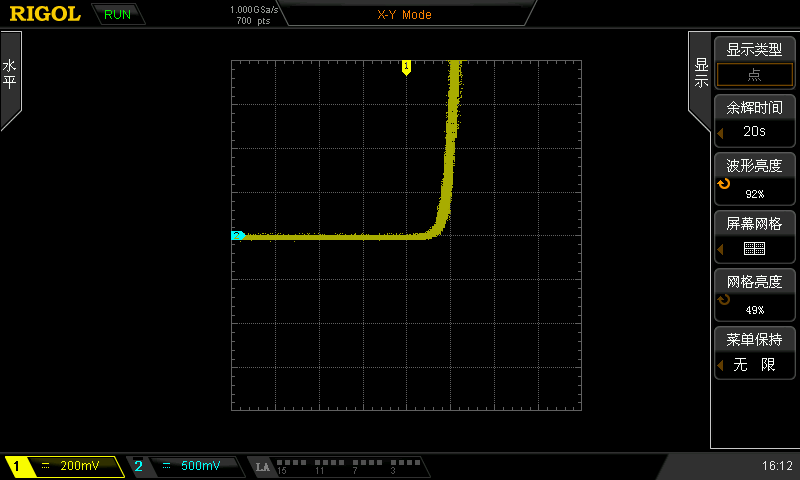
\includegraphics[width=\columnwidth]{LCE-01-二极管/assets/二极管伏安特性曲线/1N5819 Schottky.png}
    \caption{1N5819 (Schottky) 伏安特性曲线, $R_{sense} = 1 \ \mathrm{k}\Omega$}
\end{figure}

\begin{figure}[H]\centering
    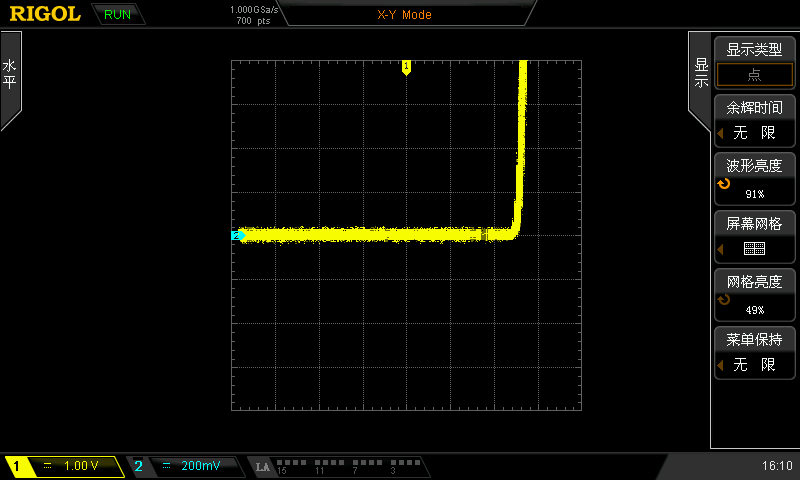
\includegraphics[width=\columnwidth]{LCE-01-二极管/assets/二极管伏安特性曲线/LED Blue.png}
    \caption{LED (Blue) 伏安特性曲线, $R_{sense} = 1 \ \mathrm{k}\Omega$}
\end{figure}

\begin{figure}[H]\centering
    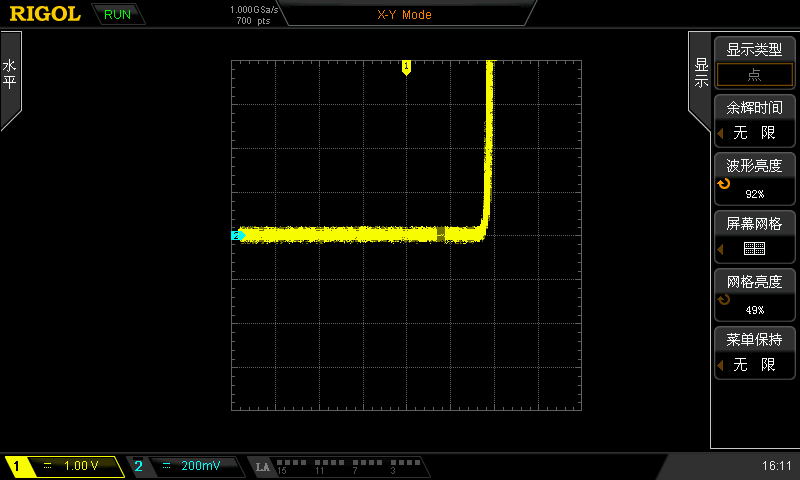
\includegraphics[width=\columnwidth]{LCE-01-二极管/assets/二极管伏安特性曲线/LED Green.png}
    \caption{LED (Green) 伏安特性曲线, $R_{sense} = 1 \ \mathrm{k}\Omega$}
\end{figure}

从图中可以看出, 1N55819 (Schottky), LED (Blue) 和 LED (Green) 的导通压降分别约为 200 mV, 2.8 V, 和 1.9 V 。这个数据与前面表 \ref{二极管导通压降实验数据} 数据有一些出入,是因为我们在伏安特性曲线的测量中,二极管的正向电流没有超过 2 mA 。1N55819 (Schottky) 为 0 $\sim$ 2 mA , LED (Blue) 和 LED (Green) 为 0 $\sim$ 0.8 mA 。

\subsection{半波整流电路 (不接输出储能电容)}

半波整流电路如图 \ref{fig: half-wave rectifier circuit} 所示,信号源通过变压器隔离后从电路的 1、2 两个输入口输入。

由于二极管的单向导电性,只有二极管处在正偏压时会产生输出电压,即输入 1 电位高于输入 2 的半周会有输出电压,其余时间输出电压为零。并且,二极管存在正向压降,因此实际输出电压比输入电压低一个导通压降。

\begin{figure}[H]\centering
    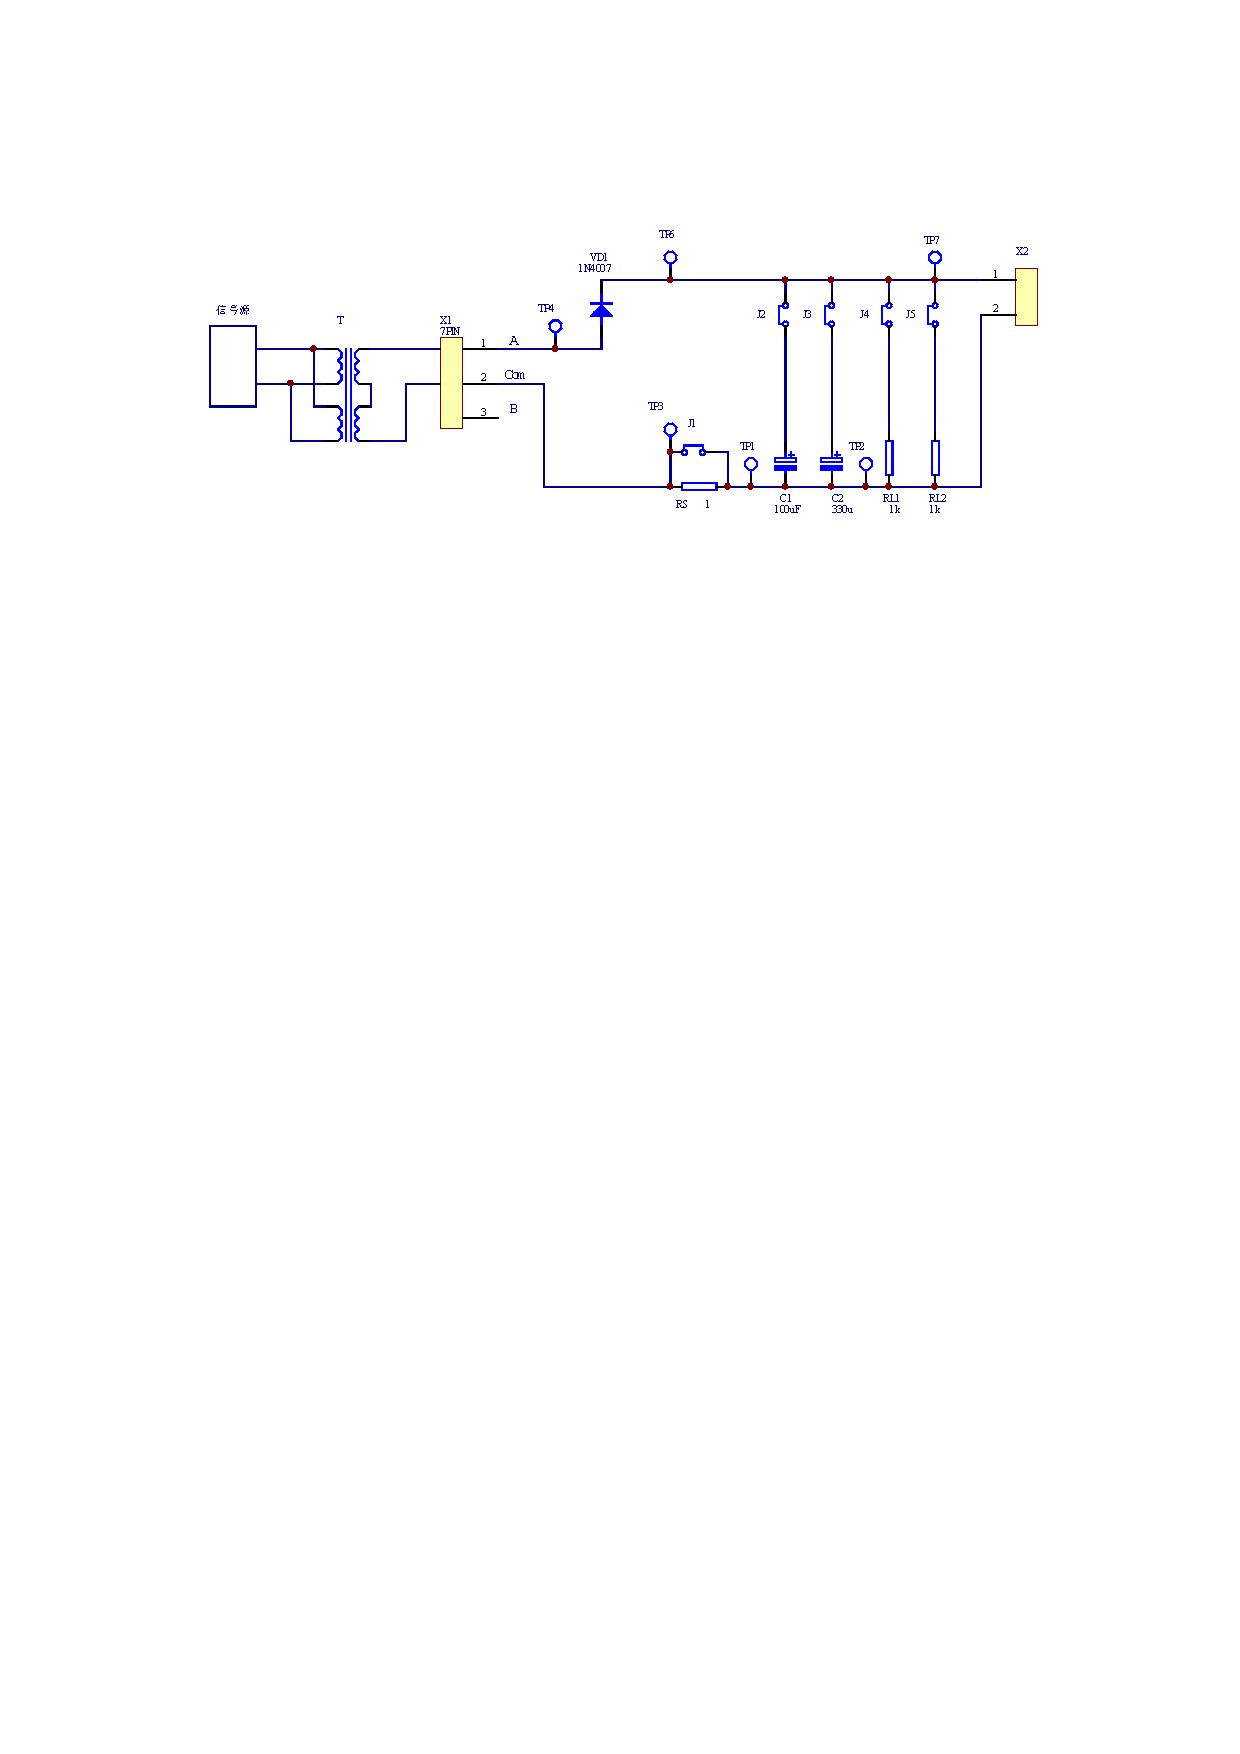
\includegraphics[width=0.9\columnwidth]{LCE-01-二极管/assets/实验原理/电路图 copy.pdf}
    \caption{半波整流电路}
    \label{fig: half-wave rectifier circuit}
\end{figure}

未连接输出储能电容时,二极管电压和输出电压波形、输出电流波形如下图所示(负载正常连接):

\begin{figure}[H]\centering
    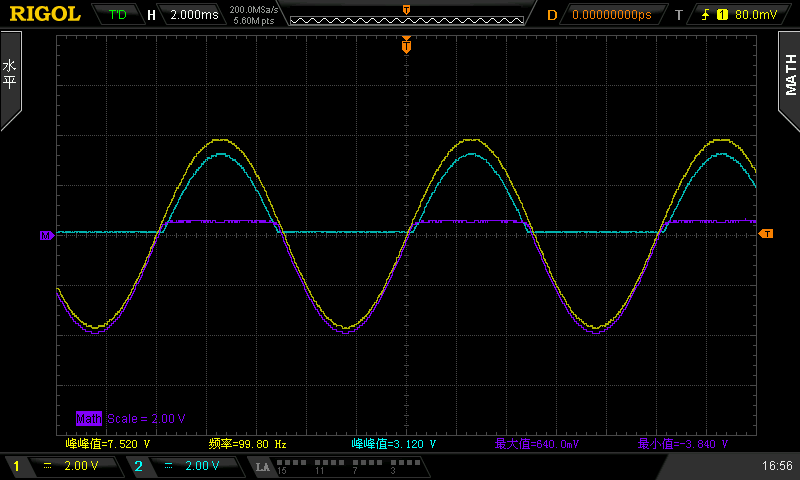
\includegraphics[width=\columnwidth]{LCE-01-二极管/assets/二极管整流电路/半波整流 单二极管 无电容 输出解电阻.png}
    \caption{半波整流 (无电容): 输入电压 (CH1, yellow)、输出电压 (CH2, blue) 和二极管正向电压 (Math, Purple)}
\end{figure}

\begin{figure}[H]\centering
    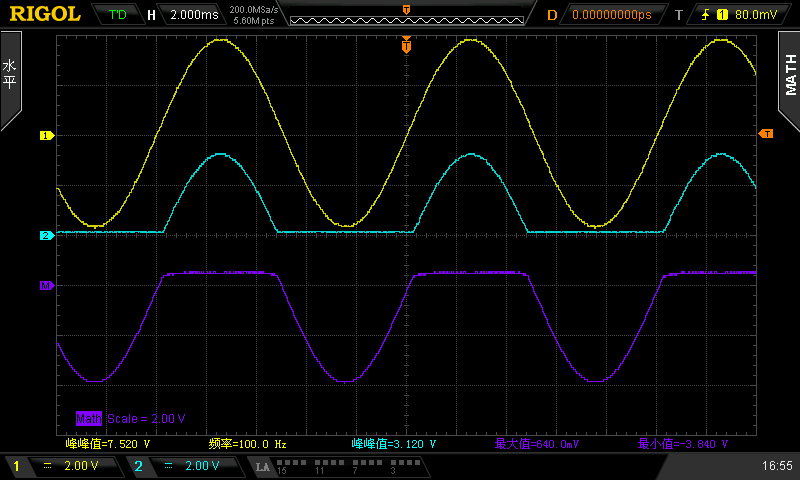
\includegraphics[width=\columnwidth]{LCE-01-二极管/assets/二极管整流电路/半波整流 单二极管 无电容 输出解电阻 (错位).png}
    \caption{半波整流 (无电容): 输入电压 (CH1, yellow)、输出电压 (CH2, blue) 和二极管正向电压 (Math, Purple), 错位显示}
\end{figure}

从图中可以看到,二极管仅在正半周期导通,且输出电压比输出电压低一个 $V_D$。


\begin{figure}[H]\centering
    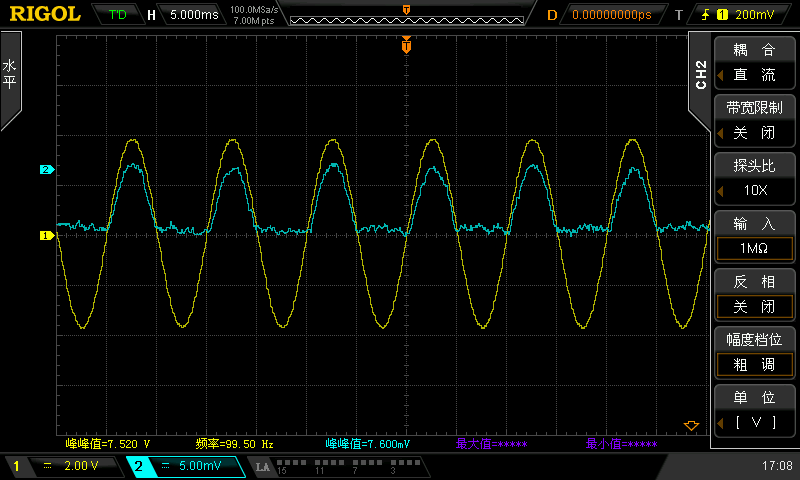
\includegraphics[width=\columnwidth]{LCE-01-二极管/assets/二极管整流电路/半波整流-电流波形 二极管 无电容 输出解电阻.png}
    \caption{半波整流 (无电容): 输入电压 (CH1, yellow)、输出电流 (CH2, blue, $R_{sense} = 1\ \Omega$)}
\end{figure}



\subsection{半波整流电路 (连接输出储能电容)}

连接输出储能电容后,输出电压的波形不再是单纯的半波整流波形,而是在半波整流波形的基础上,增加了电容充放电的过程。

\begin{figure}[H]\centering
    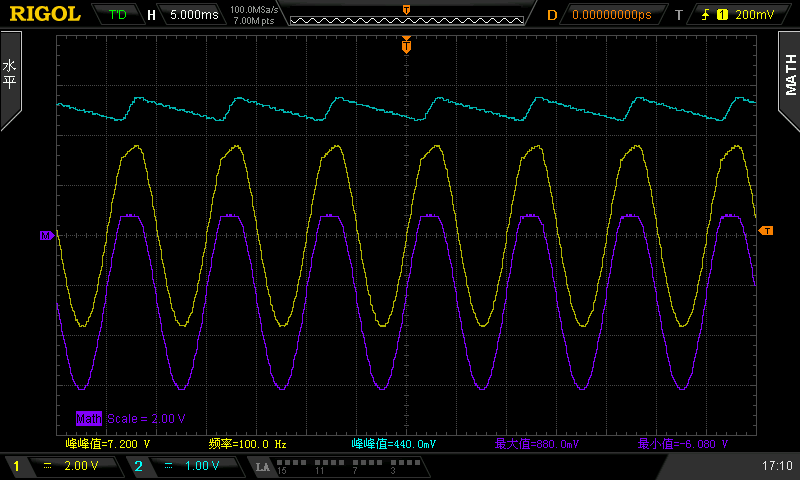
\includegraphics[width=\columnwidth]{LCE-01-二极管/assets/二极管整流电路/半波整流-接电容 单二极管 有电容 输出接电阻.png}
    \caption{半波整流 (有电容): 输入电压 (CH1, yellow)、输出电压 (CH2, blue) 和二极管正向电压 (Math, Purple), 错位显示}
\end{figure}

\begin{figure}[H]\centering
    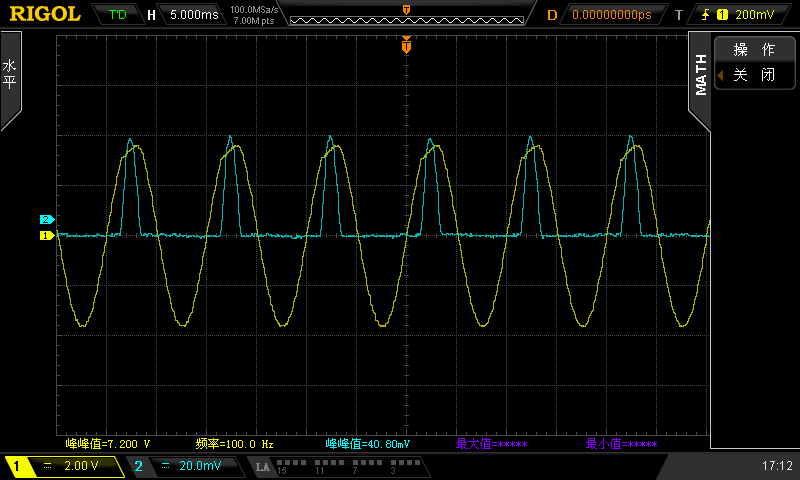
\includegraphics[width=\columnwidth]{LCE-01-二极管/assets/二极管整流电路/半波整流-接电容-电流波形 单二极管 有电容 输出接电阻.png}
    \caption{半波整流 (有电容): 输入电压 (CH1, yellow)、输出电流 (CH2, blue, $R_{sense} = 1\ \Omega$)}
\end{figure}

信号源给电容充电时,电容两端电压跟随输入电压上升(输出电压上升);电容放电时,电容两端电压下降,信号源输出电流为零。

\subsection{全波整流电路 (选做)}

全波整流的实现需要使用到“中间抽头变压器”,我们的变压器可以满足这个条件,按下图正确连接变压器输出后,对整流情况进行观察。

\begin{figure}[H]\centering
    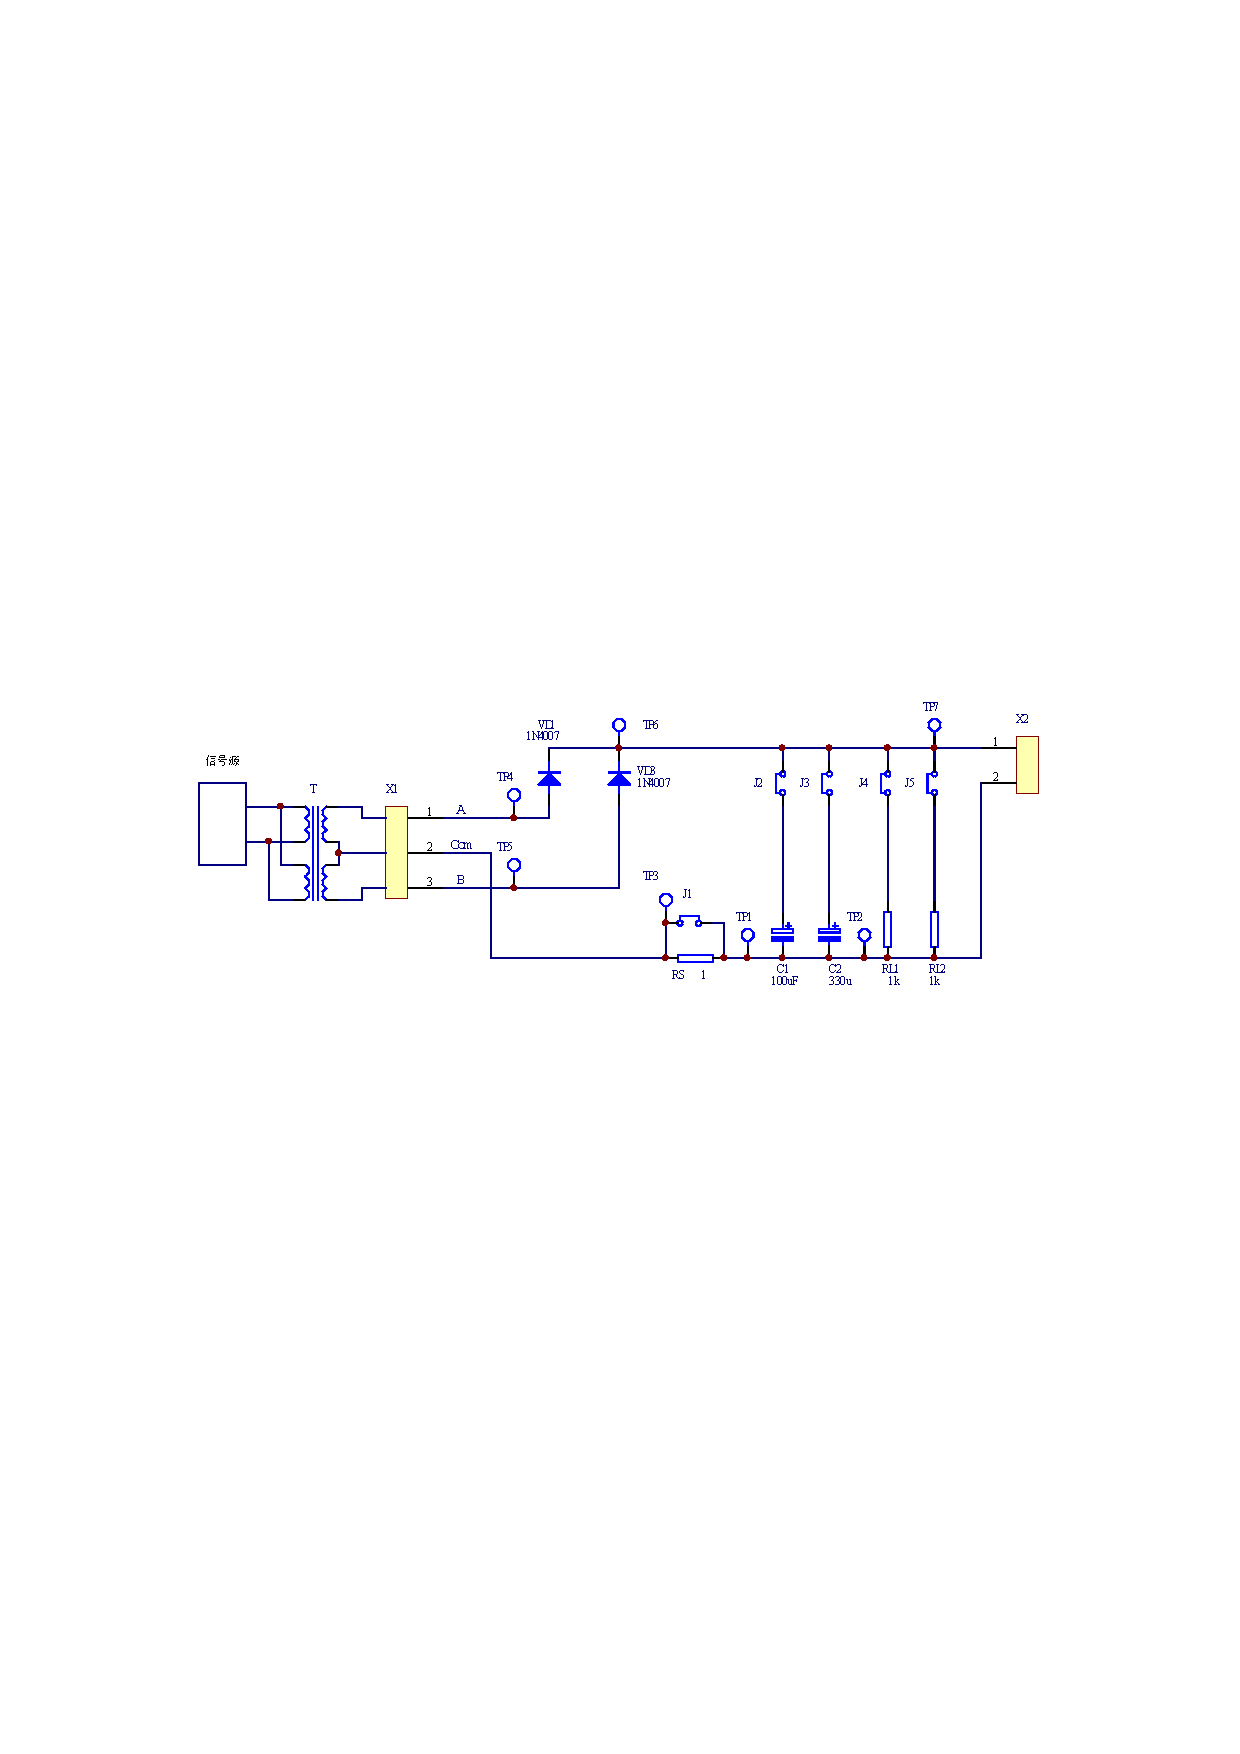
\includegraphics[width=0.9\columnwidth]{LCE-01-二极管/assets/实验原理/电路图 copy 2.pdf}
    \caption{全波整流电路}
    \label{fig: full-wave rectifier circuit}
\end{figure}

未接入储能电容时,全波整流电路的波形如下:

\begin{figure}[H]\centering
    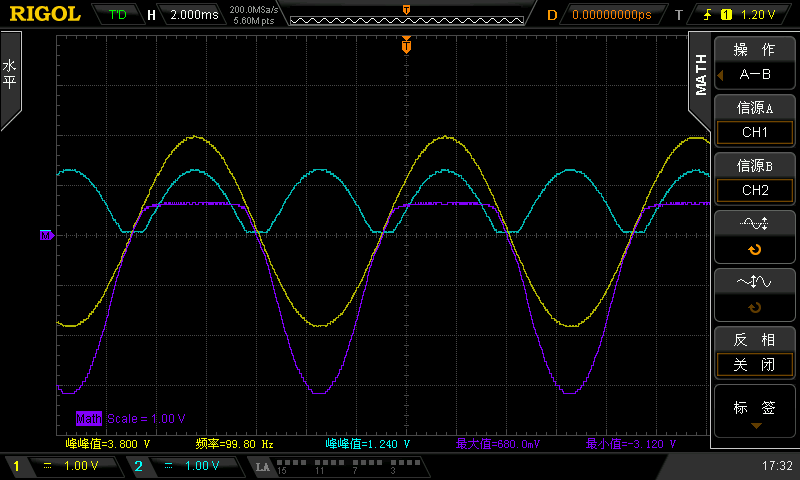
\includegraphics[width=\columnwidth]{LCE-01-二极管/assets/二极管整流电路/全波整流-无电容-电压波形.png}
    \caption{全波整流 (无电容): 输入电压 (CH1, yellow)、输出电压 (CH2, blue) 和二极管正向电压 (Math, Purple)}
\end{figure}


\begin{figure}[H]\centering
    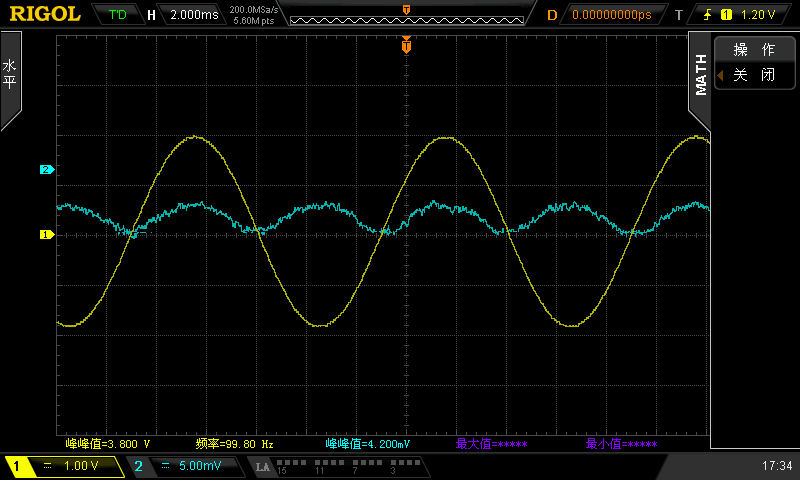
\includegraphics[width=\columnwidth]{LCE-01-二极管/assets/二极管整流电路/全波整流-无电容-电流波形.png}
    \caption{全波整流 (无电容): 输出电压 (CH1, yellow)、输出电流 (CH2, blue, $R_{sense} = 1\ \Omega$)}
\end{figure}

由图可以看出,二极管在正负两个半周期都能够导通,输出电压波形为全波整流波形。但是由于二极管存在导通压降,输出波形仍存在“死区”电压,此时两个二极管都未导通,输出电压为零。

将储能电容重新接入,输出波形如下:

\begin{figure}[H]\centering
    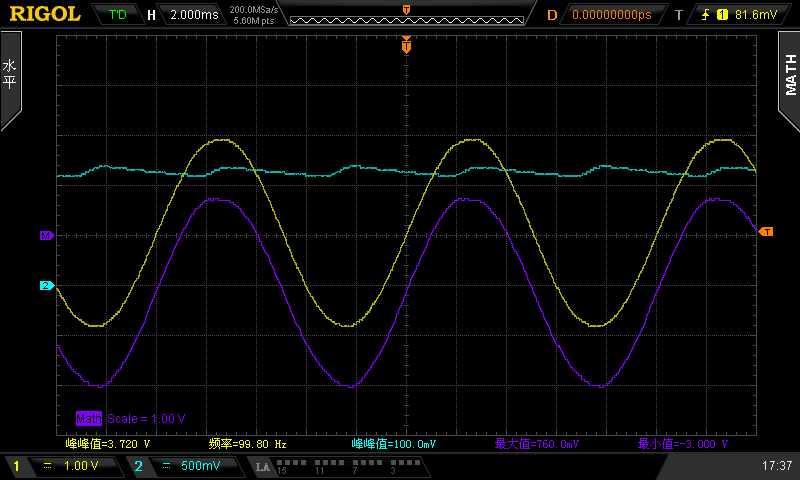
\includegraphics[width=\columnwidth]{LCE-01-二极管/assets/二极管整流电路/全波整流-接电容-电压波形.png}
    \caption{全波整流 (有电容): 输入电压 (CH1, yellow)、输出电压 (CH2, blue) 和二极管正向电压 (Math, Purple)}
\end{figure}

\begin{figure}[H]\centering
    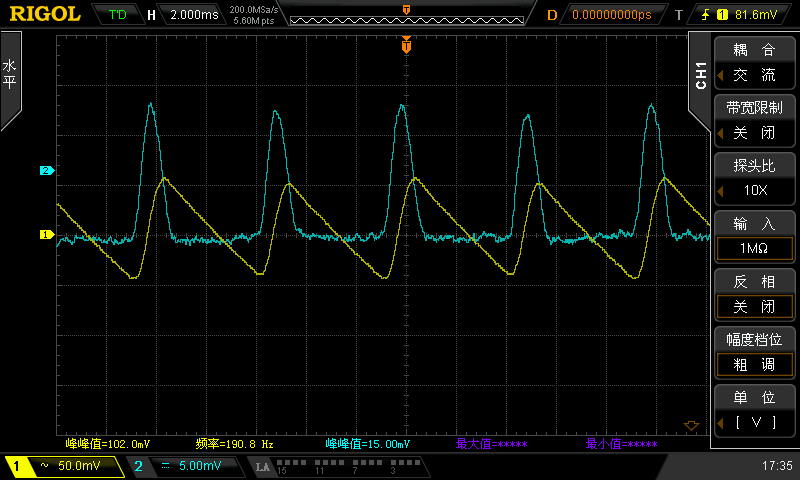
\includegraphics[width=\columnwidth]{LCE-01-二极管/assets/二极管整流电路/全波整流-接电容-电流波形.png}
    \caption{全波整流 (有电容): 输出电压 (CH1, yellow, ac coupling)、输出电流 (CH2, blue, $R_{sense} = 1\ \Omega$)}
\end{figure}

与半波整流相比,输出纹波的频率变为了输入频率的两倍,且纹波幅度明显减小,这是因为全波整流电路在每个半周期都能够给储能电容充电。

\subsection{桥式整流电路 (选做)}

实际中最常用的整流电路是桥式整流,实验电路图如下:

\begin{figure}[H]\centering
    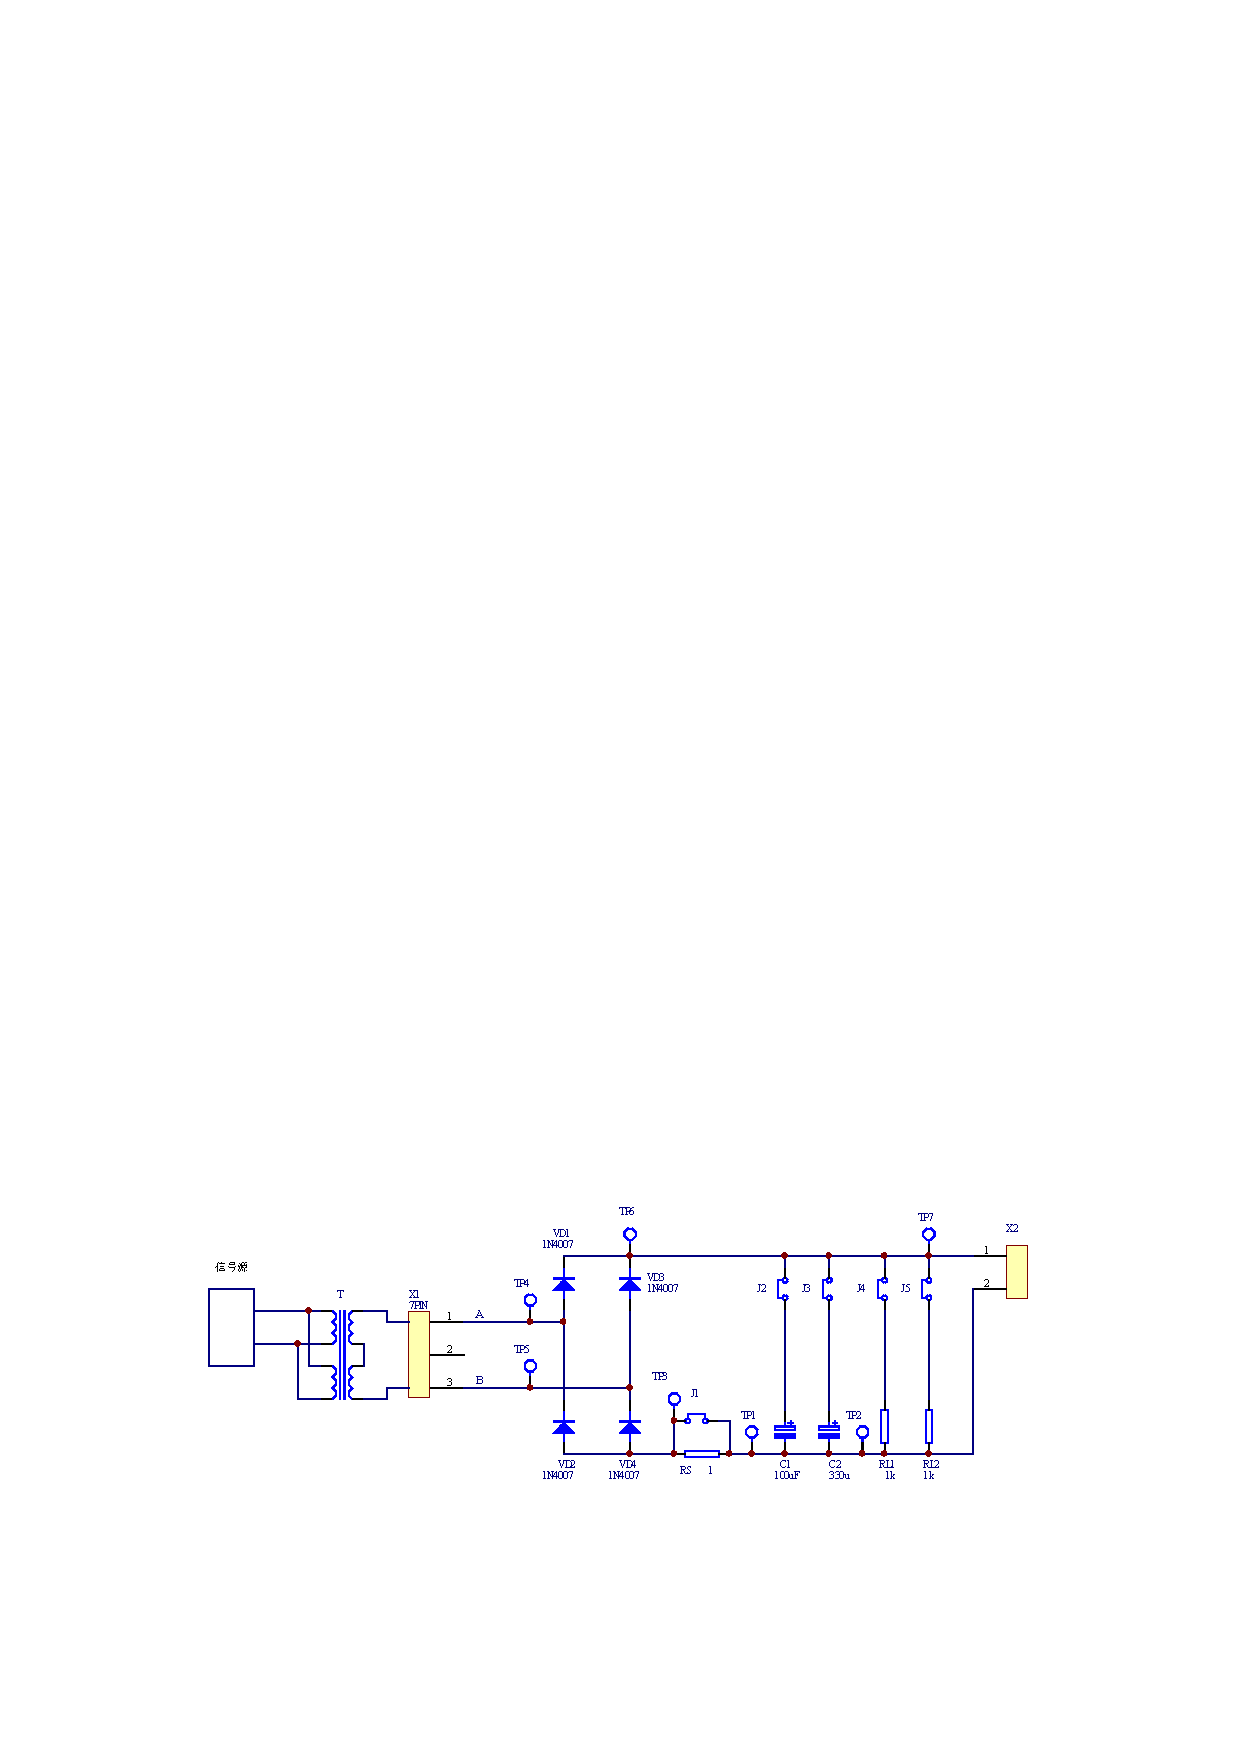
\includegraphics[width=0.9\columnwidth]{LCE-01-二极管/assets/实验原理/电路图 copy 3.pdf}
    \caption{桥式整流电路}
    \label{fig: bridge rectifier circuit}
\end{figure}

接入小储能电容时 ($100 \ \mathrm{\mu F}$),桥式整流电路的波形如下:

\begin{figure}[H]\centering
    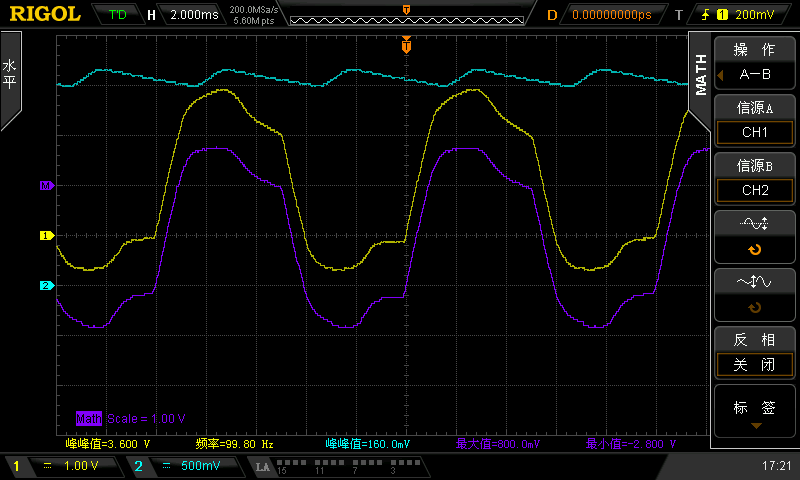
\includegraphics[width=\columnwidth]{LCE-01-二极管/assets/二极管整流电路/桥式整流-接电容-电压波形.png}
    \caption{桥式整流 (小电容): 输入电压 (CH1, yellow)、输出电压 (CH2, blue) 和二极管正向电压 (Math, Purple)}
\end{figure}

\begin{figure}[H]\centering
    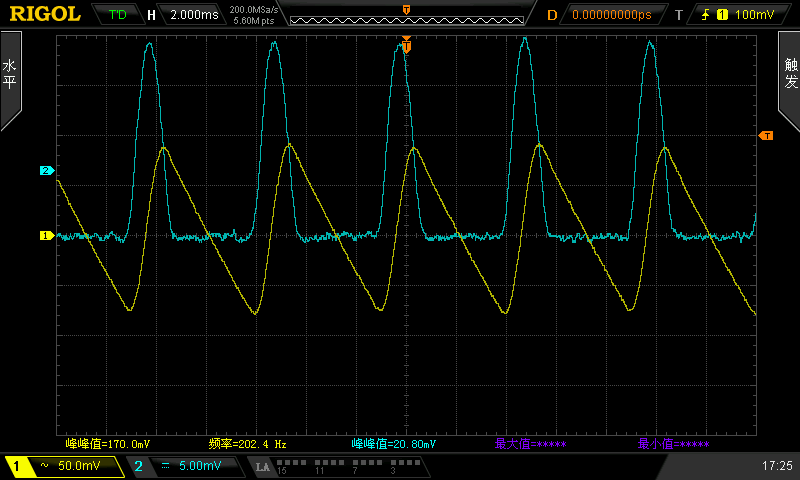
\includegraphics[width=\columnwidth]{LCE-01-二极管/assets/二极管整流电路/桥式整流-接电容-电流波形.png}
    \caption{桥式整流 (小电容): 输出电压 (CH1, yellow)、输出电流 (CH2, blue, $R_{sense} = 1\ \Omega$)}
\end{figure}

同时接入小电容和大电容时 ($100 \ \mathrm{\mu F} + 330 \ \mathrm{\mu F}$),桥式整流电路的输出电压电流波形如下图所示。纹波幅度明显降低,输出电压更加平稳。

\begin{figure}[H]\centering
    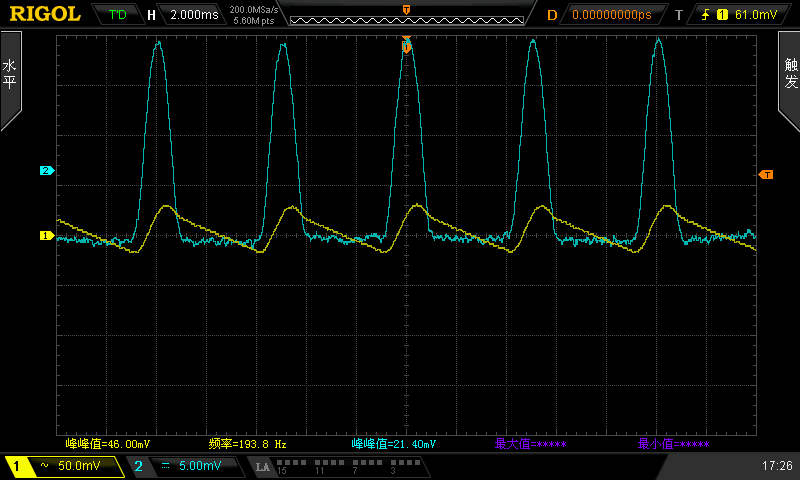
\includegraphics[width=\columnwidth]{LCE-01-二极管/assets/二极管整流电路/桥式整流-接大电容-电流波形.png}
    \caption{桥式整流 (小电容 + 大电容): 输出电压 (CH1, yellow)、输出电流 (CH2, blue, $R_{sense} = 1\ \Omega$)}
\end{figure}


\subsection{二极管反向恢复特性 (选做)}


二极管在快速关闭时,存在“反向恢复时间”的概念。在这段极短的时间内,二极管的压降比 0 V 稍低,但是反向电流却很大(类似一个阻值很低的电阻),这个现象在需要频繁开关的场合可能会产生较大损耗。


\begin{figure}[H]\centering
    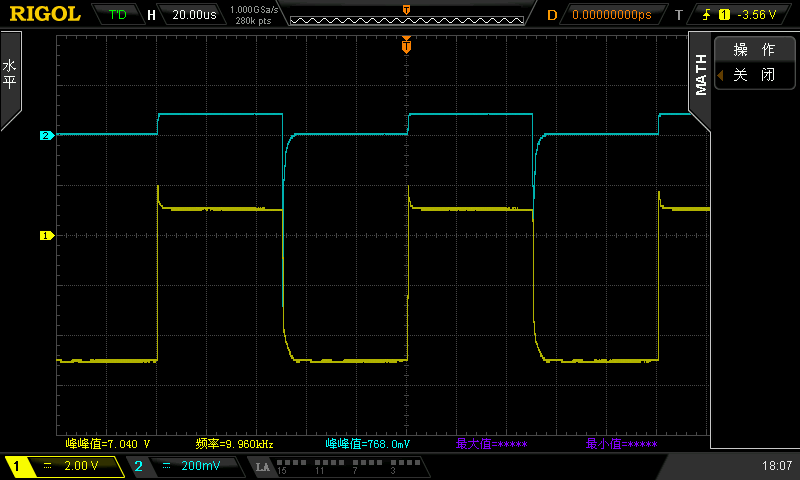
\includegraphics[width=\columnwidth]{LCE-01-二极管/assets/二极管反相恢复特性/二极管反相恢复特性 1Ohm电阻 1N4007 10KHz.png}
    \caption{二极管反向恢复特性:二极管正向压降 (CH1, yellow)、二极管正向电流 (CH2, blue, $R_{sense} = 1 \Omega$)}
    \label{fig: 二极管反向恢复特性}
\end{figure}

由于信号源输出电流有限,无法观察到反相恢复特性,我们利用 TC4424 功率驱动芯片,对信号源输出的方波进行功率放大。设置 TC4424 输出 10 kHz 的方波,对二极管 1N4007 进行测试,结果见图 \ref{fig: 二极管反向恢复特性} 和图 \ref{fig: 二极管反向恢复特性 细节放大}。

\begin{figure}[H]\centering
    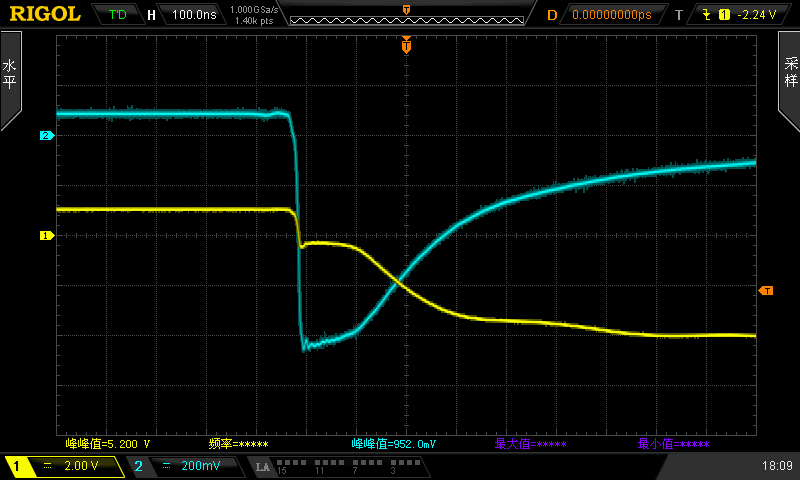
\includegraphics[width=\columnwidth]{LCE-01-二极管/assets/二极管反相恢复特性/二极管反相恢复特性-细节放大 1Ohm电阻 1N4007 10KHz.png}
    \caption{二极管反向恢复特性:二极管正向压降 (CH1, yellow)、二极管正向电流 (CH2, blue, $R_{sense} = 1 \Omega$), 细节放大}
    \label{fig: 二极管反向恢复特性 细节放大}
\end{figure}

由图中可以看到,在二极管电压下降,二极管从开启到关闭的过程中,二极管的电流并不是瞬间变为零,而是在 200 ns $\sim$ 400 ns 的反向放电之后,才逐渐减小至零。这个反向恢复时间是比较正常的,因为 1N4007 只是一种通用整理二极管。

\section{思考题}

\subsection*{4.1 \ \ 对本实验的建议}

此次实验有较多的选做部分,同学们可以根据自己的安排、兴趣任意选择。但是选做实验的实验原理、实验步骤,课件和相关实验资料中并没有详细说明,希望能补上这一部分内容,以便想完成选做实验的同学参考。

\subsection*{4.2 \ \ 二极管接入滤波电容后,输入输出有哪些主要变化?有无负面影响?}

整流电路中的滤波电容(即储能电容)能够对整流后的脉动电压进行平滑处理,使输出电压波形更加平滑,脉动成分减小。滤波电容的存在使得输出电压的平均值有所提高,并且二极管的导通时间变短,只有在输入电压大于电容两端电压时,才有电流对电容充电和对负载供电。

最大的负面影响时,加入电容后,电容储能(产生电压),二极管的正极被拉高到输出电压,导致整流过程中二极管承受的最大反向电压变为原来的两倍,这对二极管的耐压有了更高的要求。另一个可能的负面影响是,由于电容滤波的作用,二极管在充电瞬间需要提供较大的电流,导致电流峰值增大,这可能会对二极管的耐流能力提出更高要求。

\subsection*{4.3 \ \ 逐点法测量伏安特性,主要误差有哪些?}

\noindent 主要的误差有以下几点:
\begin{enumerate}
\item 系统误差:采用电流表外接法时,电压表测量的是二极管与电流表两端的电压之和,导致测得的电压偏大;而电流表内接时,电流表测量的是通过二极管和电压表的总电流,导致测得的电流偏大;
\item 环境因素:二极管的特性参数(如正向导通电压、反向漏电流等)会随温度变化而改变,测量过程中的温度变化会对测量结果产生影响;
\item 读数误差:人为读取电压表和电流表数值时,可能会因仪器精度、示数波动等因素导致读数不准确;
\end{enumerate}

下面进行一些定量的计算。考虑我们所使用的测量方法 (DC Power Supply + 1 $\mathrm{k}\Omega$ 电阻),查阅资料\footnote{电源技术指标在 \href{http://www.gwinstek.com.cn/product/detail/195}{http://www.gwinstek.com.cn/product/detail/195},万用表技术指标在 \href{https://meters.uni-trend.com.cn/list\_40/123.html}{https://meters.uni-trend.com.cn/list\_40/123.html}}知电源电压的“读值精确度”为 ±(0.03 \% 的读数 + 10 位) ,万用表电压读数精度为 ±(0.05\% + 5 位) 测量得到万用表电压档的内阻约为 11 $\mathrm{M}\Omega$,电阻精度为 ± 1 \%。

假设现在电源输出的电压读数为 10 V, 万用表电压读数为 2 V, 忽略误差下的测量结果为:
\begin{gather}
(V_D,\ I_D) = (2 \mathrm{V},\ 8 \ \mathrm{mA})
\end{gather}
考虑仪器带来的误差,实际测量点可能为:
\begin{gather}
    2 \mathrm{V} \times 0.05\, \% = 1.0 \ \mathrm{mV}, \quad 
    10 \mathrm{V} \times 0.03\, \% = 3.0 \ \mathrm{mV}
    \\
    \frac{
        (10 \mathrm{V} \pm 3.0 \ \mathrm{mV}) - (2 \mathrm{V} \pm 1.0 \ \mathrm{mV})
        }{
        1 \mathrm{k}\Omega \pm 10 \ \Omega
    } \in [8 \ \mathrm{mA}- 0.0832 \ \mathrm{mA},\  8 \ \mathrm{mA} + 0.0848 \ \mathrm{mA}] 
    \\
    \Longrightarrow 
(V_D,\ I_D) = (2 \ \mathrm{V} \pm 0.6 \ \mathrm{mV},\ 8 \ \mathrm{mA} \pm 0.09 \ \mathrm{mA})
\end{gather}
显然,电流上的误差相对较大,最大可能达到 $1.125 \%$ 左右。

\subsection*{4.4 \ \ 计算变压器次级等效源阻抗}

设变压器原副边变比为 $n$,原边电源的输出阻抗为 $Z_s$,则对副边而言,原边带来的等效源阻抗为:
\begin{gather}
    Z_{eq} = \frac{Z_s}{n^2}
\end{gather}

\subsection*{能否用实验室信号源、变压器、二极管产生 700V 直流电压?}

实验室的变压器最大匝数比可以为 $\frac{220}{20.3} \approx 11$,两个信号源的输出幅度最大为 40 Vpp ,因此最大只能升压到约 440 Vpp 。要想产生 700 V 的直流电压,需要更大的变压器匝数比,或者再加入一个电压倍增器。

\section{异常现象分析}

实验中,绝大多数现象都是符合预期的,但是我使用的示波器似乎有一些问题。具体现象是,在默认参数下,将 CH2 探头正极与负极直接连接,此时示波器 CH2 的值会有约 -5 mV 至 -10 mV 的“偏移”,如下图所示:

\begin{figure}[H]\centering
    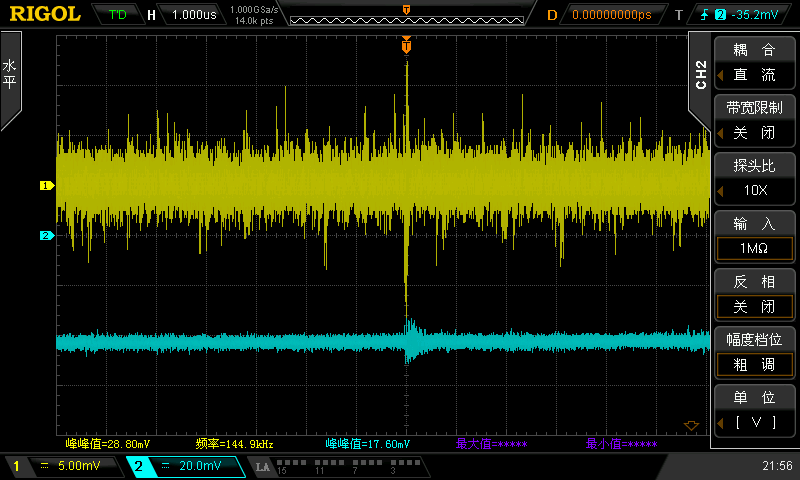
\includegraphics[width=\columnwidth]{LCE-01-二极管/assets/异常分析/示波器 CH2 的偏移现象.png}
    \caption{示波器 CH2 的“偏移”现象}
\end{figure}

作为对比,我们在上图中将 CH1 的探头也短接到了地。显然, CH1 的测量结果没有发生偏移。我们尝试过交换示波器的探头、将示波器模式调整为“高分辨率”、将示波器触发源改为 CH1,异常现象都没有明显变化。除此之外,我对邻桌的的示波器进行了测试,也出现了相同的现象,只不过偏移幅度略有不同。

上面问题的一个伴生现象是,将示波器的触发源调整为 CH2,然后向下移动触发电平,会发现 CH2 的值也向下移动(始终比触发电平低 10 mV 左右)。因此,我猜测,这是 RIGOL MSO2202A CH2 通道采样上的设计问题,是普遍存在的系统问题。























































































































\newpage
% 附录 A
\section*{附录 A\hspace*{20pt} 预习报告}
\addcontentsline{toc}{section}{附录 A\hspace*{6pt} 预习报告} 
\thispagestyle{fancy} 
\begin{figure}[H]\centering
    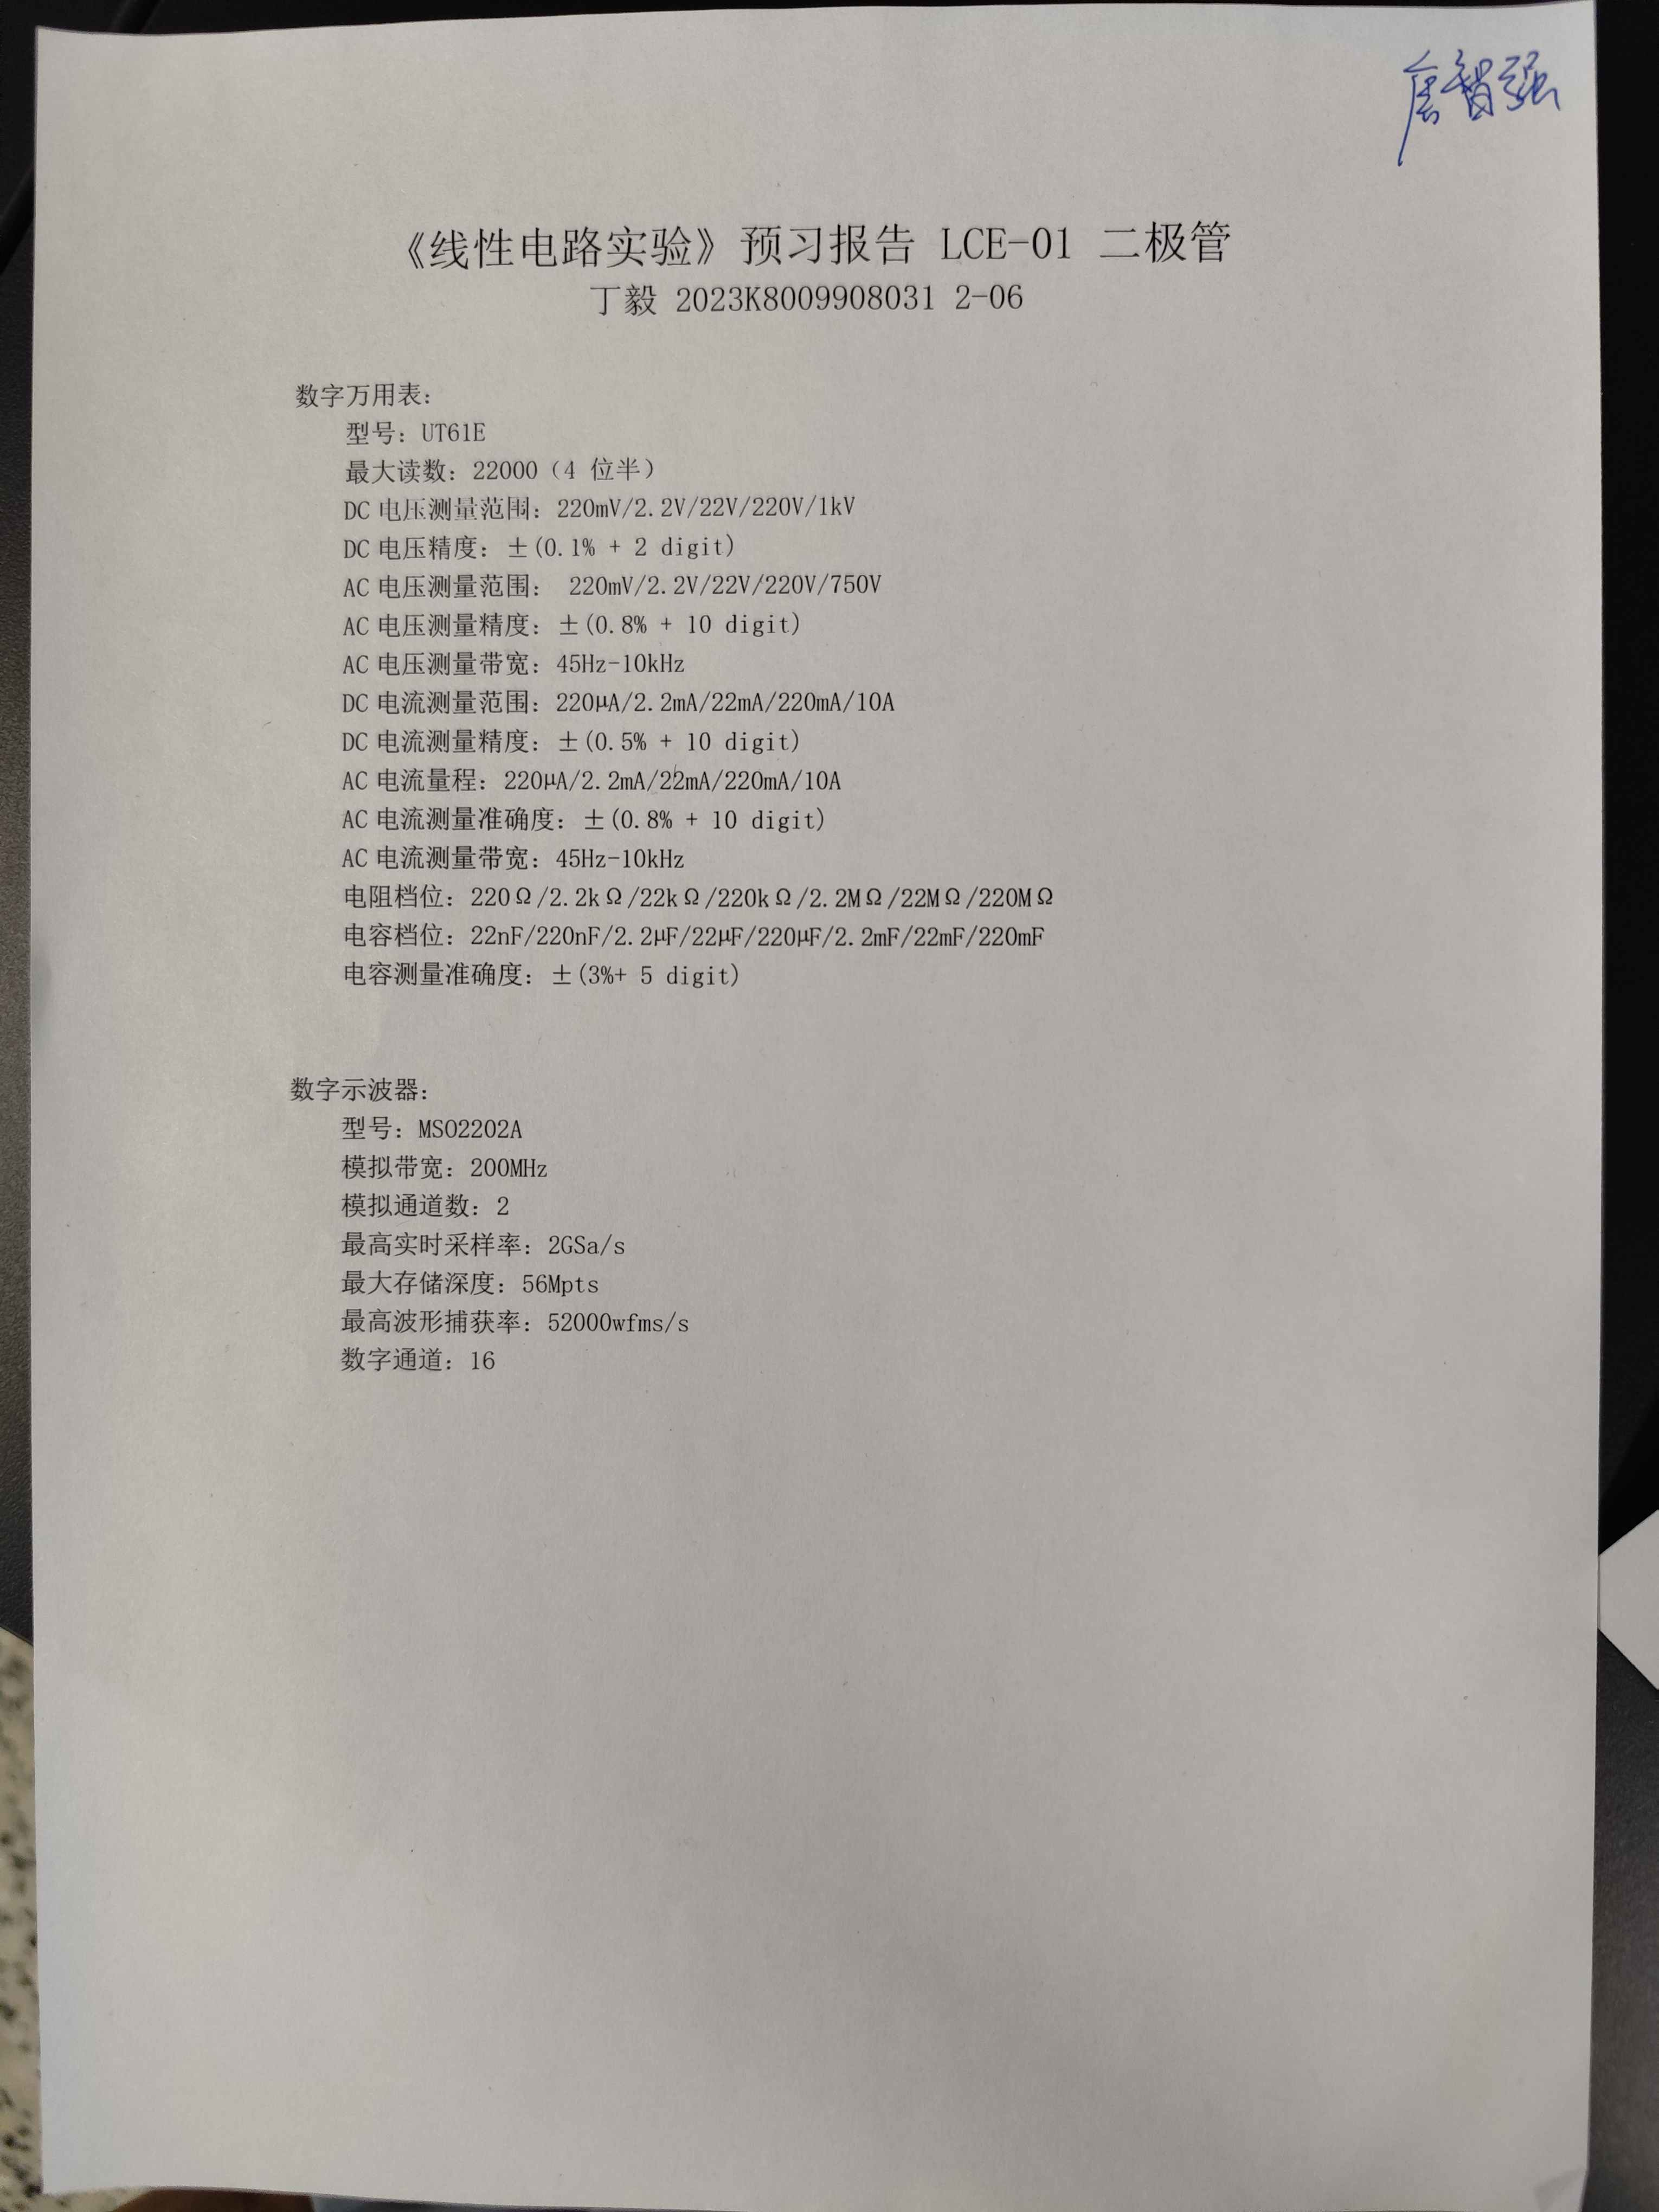
\includegraphics[width=\columnwidth]{LCE-01-二极管/assets/预习报告.jpg}
    \caption{预习报告}
\end{figure}

% 附录 B
\section*{附录 B\hspace*{20pt} 原始数据记录表}
\addcontentsline{toc}{section}{附录 B\hspace*{6pt} 原始数据记录表} 
\thispagestyle{fancy} 

\begin{figure}[H]\centering
    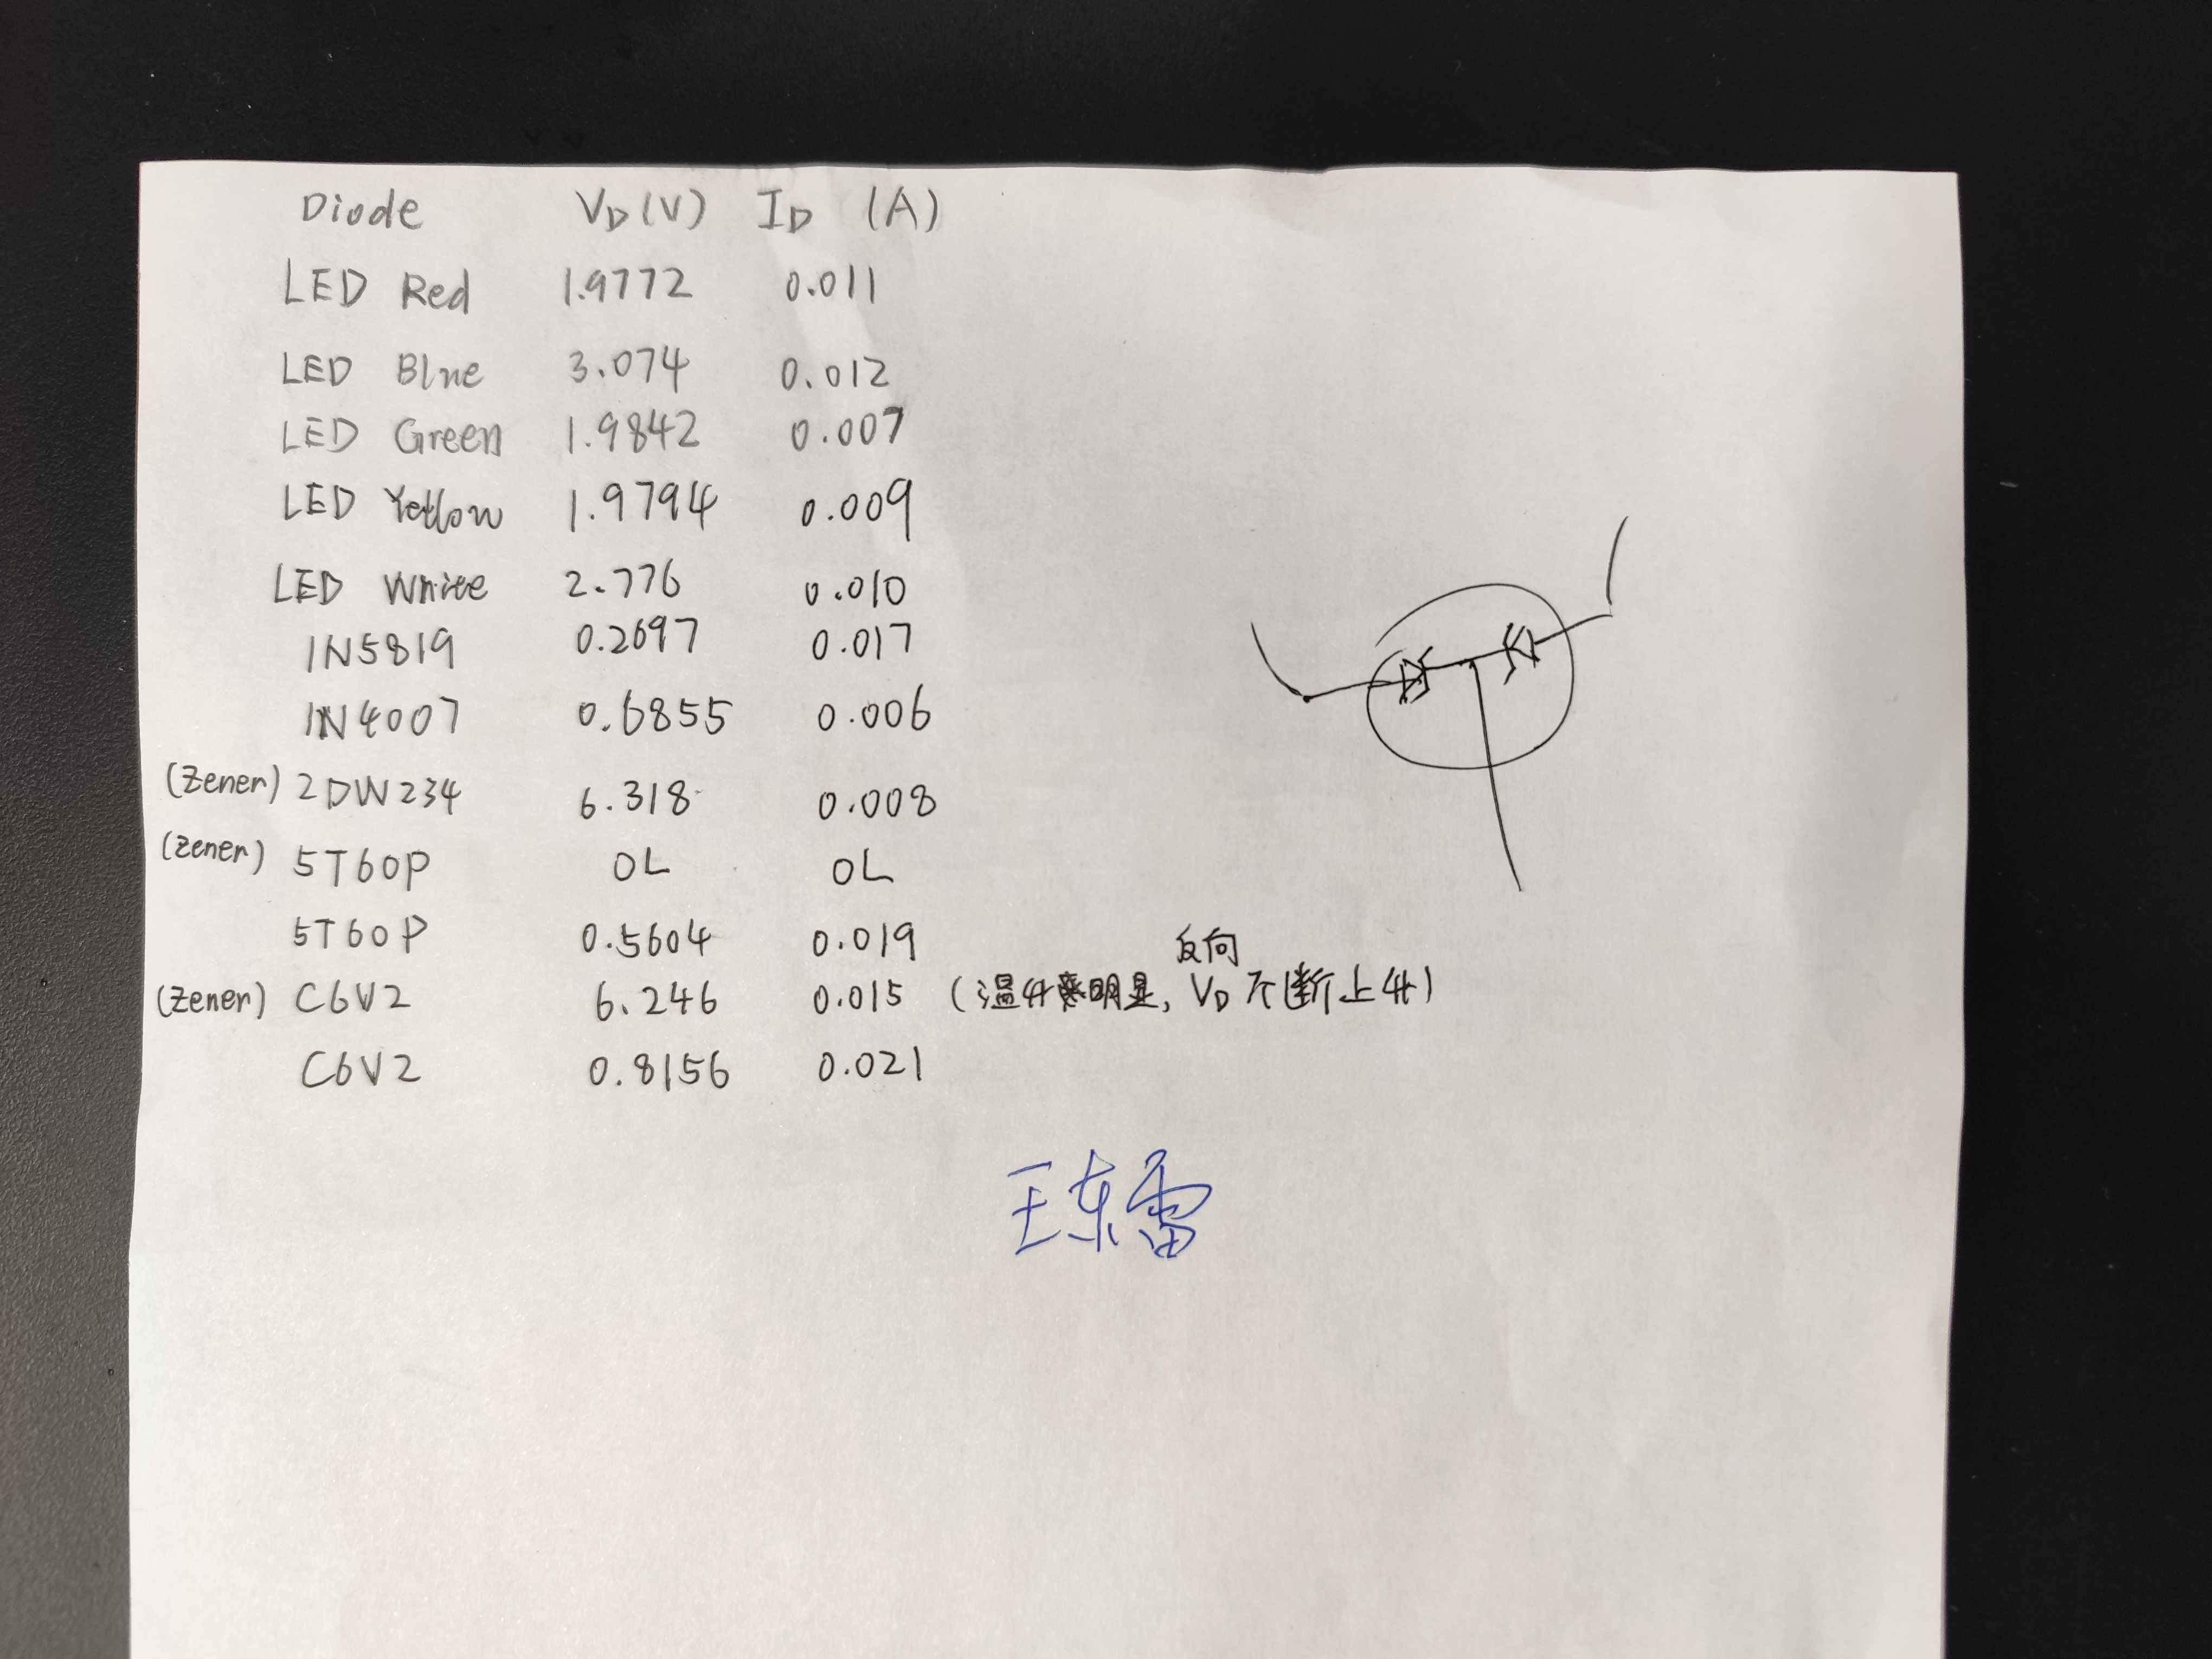
\includegraphics[width=\columnwidth]{LCE-01-二极管/assets/原始数据.jpg}
    \caption{原始数据记录表}
\end{figure}

% 附录
%\section*{附录 C \hspace*{20pt} Matlab Codes}
%\addcontentsline{toc}{section}{附录 C \hspace*{6pt} Matlab Codes} 
%\thispagestyle{fancy} 
%\lstinputlisting{d:/a_RemoteRepo/GH.MatlabCodes/本科课程代码/基础物理实验/Ex_9/Ex_9_analysis_mfile.m}



\end{document}

% VScode 常用快捷键:

% F2:                       变量重命名
% Ctrl + Enter:             行中换行
% Alt + up/down:            上下移行
% 鼠标中键 + 移动:           快速多光标
% Shift + Alt + up/down:    上下复制
% Ctrl + left/right:        左右跳单词
% Ctrl + Backspace/Delete:  左右删单词    
% Shift + Delete:           删除此行
% Ctrl + J:                 打开 VScode 下栏(输出栏)
% Ctrl + B:                 打开 VScode 左栏(目录栏)
% Ctrl + `:                 打开 VScode 终端栏
% Ctrl + 0:                 定位文件
% Ctrl + Tab:               切换已打开的文件(切标签)
% Ctrl + Shift + P:         打开全局命令(设置)

% Latex 常用快捷键:

% Ctrl + Alt + J:           由代码定位到PDF


